\documentclass{beamer}
%\documentclass[handout,t]{beamer}

\batchmode
% \usepackage{pgfpages}
% \pgfpagesuselayout{4 on 1}[letterpaper,landscape,border shrink=5mm]

\usepackage{amsmath,amssymb,enumerate,epsfig,bbm,calc,color,ifthen,capt-of}
\usepackage{url} 
\usepackage{hyperref} 
\usepackage{geometry}
%\usepackage[numbers]{natbib}
\usepackage{bibentry,natbib}
\usepackage{listings}
\usepackage{alltt}
\usepackage{bigstrut}
\usepackage{array}
%\usepackage{algpseudocode}
\usepackage{algorithm}
\usepackage{algorithmic}
%\usepackage{algpseudocode}
\usepackage{float}

\usetheme{Berlin}

\newcommand{\setS}{\mathbf{G}}
\newcommand{\comp}{C}
\newcommand{\TranscodeIndicator}{P}
\newcommand{\RequestingSeg}{\mathbf{K}}
\newcommand{\TranscodeSet}{\mathbf{E}}
\newcommand{\IdleComp}{I}
\newcommand{\SegRepCost}{F}
\newcommand{\Assign}{A}
\newcommand{\ReqFromRegion}{J}
\newcommand{\CDNRegions}{\mathbf{R}}
\newcommand{\Users}{\mathbf{U}}
\newcommand{\Redirect}{D}
\newcommand{\RegionRepCost}{Z}
\newcommand{\bandwidth}{W}
\newcommand{\Version}{L}
\newcommand{\USPref}{H}
\newcommand{\ReqOfSeg}{Q}
\newcommand{\SegQuality}{Y}
\newcommand{\Bitrate}{B}

\title{A Joint Online Transcoding and Delivery Approach for Dynamic Adaptive Streaming}
\author{Alan Zhuang\\
\href{mailto:qzhuang@ust.hk}{\nolinkurl{qzhuang@ust.hk}}\\
}

%\title{$k$NN Query over a Whole Internet Topology\\\Small{and interative IP clustering and splitting}}
%\author{Alan Zhuang}
\date{\today}
\pgfdeclareimage[height=0.5cm]{ust-logo}{UST4C_L3.eps}
\logo{\pgfuseimage{ust-logo}\hspace*{0.3cm}}

\AtBeginSection[]
{
  \begin{frame}<beamer>
    \frametitle{Outline}
    \tableofcontents[currentsection]
  \end{frame}
}
\beamerdefaultoverlayspecification{<+->}
% -----------------------------------------------------------------------------
\begin{document}
% -----------------------------------------------------------------------------
\bibliographystyle{ieeetr}
\nobibliography{IEEEabrv,TMM_transcoding_delivery.bib}
%\nobibliography*%

\frame{\titlepage}

\section[Outline]{}
\begin{frame}{Outline}
  \tableofcontents
\end{frame}

% -----------------------------------------------------------------------------
\section{Background}

\begin{frame}{Challenges in the Multi-screen Era}
	\begin{itemize}
		\item<1> multiple platforms \\ %
		
\includegraphics[height=1.6cm]{fig/PCs.png}
		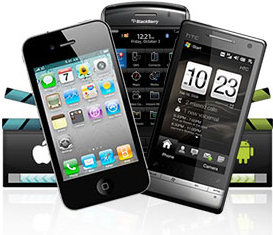
\includegraphics[height=1.0cm]{fig/mobile-bc.png}
		
\includegraphics[height=1.1cm]{fig/streaming-bc.png}
		
\includegraphics[height=1.6cm]{fig/video_quality-bc.png} 
		\item<1> multiple screen sizes \\ %
		
\includegraphics[height=1.3cm]{fig/screen_sizes.jpg}
		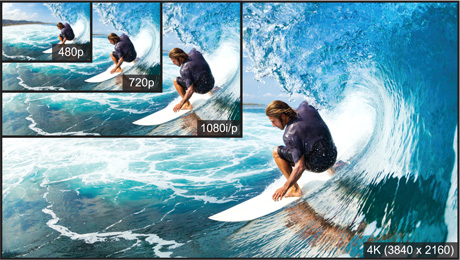
\includegraphics[height=2.1cm]{fig/480_to_4KVideo.jpg}
		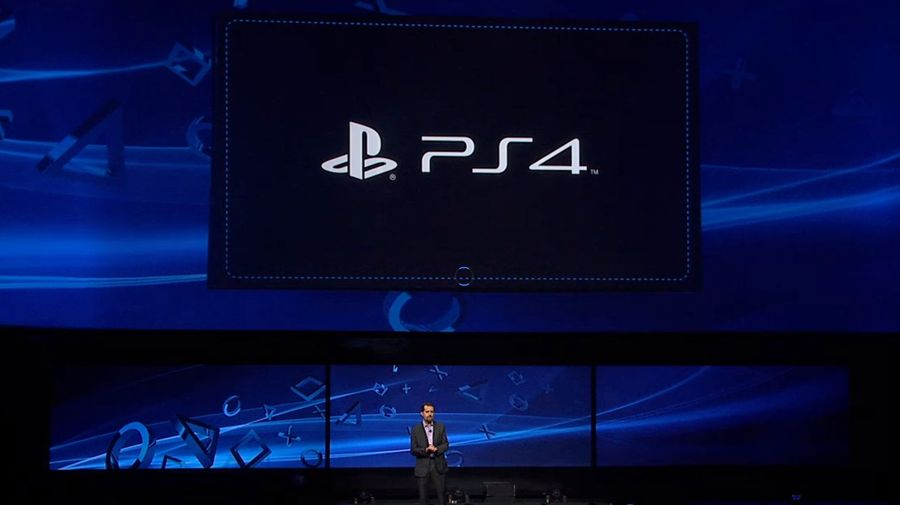
\includegraphics[height=2.1cm]{fig/4k_video.jpg} 
	\end{itemize}
\end{frame}

\begin{frame}{Challenges in the Multi-screen Era} 
	\begin{itemize}
		\item<1> different supports for containers \\ %
		mp4, mkv, avi, flv, wmv, rmvb, webm, mpeg-ts... 
		\item<1> different supports for coding standards\\ 
		H.264(AVC), H.265(HEVC), VC-1, AVS, VP8/9, RealVideo...
		
		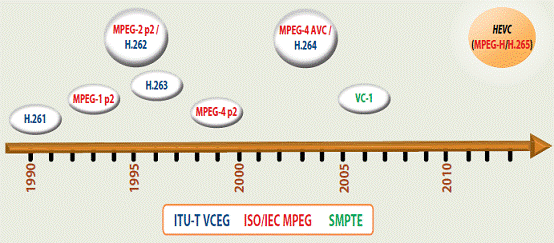
\includegraphics[height=3.5cm]{fig/encoding_standards.png}
	\end{itemize}
\end{frame}

\begin{frame}{Challenges in the Multi-screen Era} 
	\begin{itemize}
		\item<1> multiple decoding capabilities\\
		\begin{itemize}
			\item<1> $\longleftarrow$2008: MPEG4
			\item<1> $\longrightarrow$2009: H.264(AVC)
			\item<1> latest: H.265(HEVC)\\
			Apple iPhone6, Huawei Honor, Samsung Galaxy S4, Google/LG Nexus 5, XiaoMi 4, ...
		\end{itemize}
		\item<1> a hardware (chip series) example \\
			{\scriptsize
			\begin{center}
				\begin{tabular}{l|llll} %\toprule
					\hline
					MediaTek & MT6572 & MT6582 & MT6588 & MT6592 \\ %\midrule
					\hline
					Display  & 960$\times$540P & 1280$\times$720P & 1920$\times$1280P & 1920$\times$1280P \\
					H.264 Decode   & 720P@30fps & 1080P@30fps  & 1080P@30fps  & 1080P@30fps \\ 
					HEVC Decode   &  N/A &  N/A  & 720P@30fps  & 720P@30fps \\ 
					\hline
					%\bottomrule
				\end{tabular}
			}
			\end{center}	
	\end{itemize}
\end{frame}

\begin{frame}{Challenges in the Multi-screen Era} 
	\begin{itemize}
		\item<1> competitions between giants
		\begin{center}
		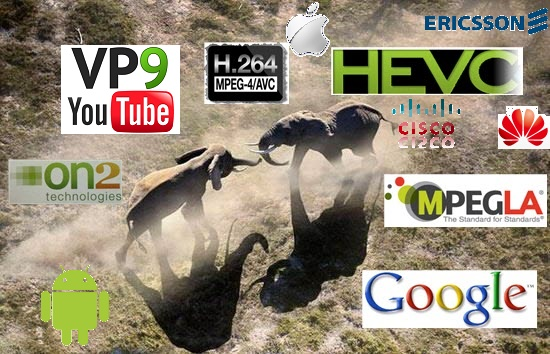
\includegraphics[height=6cm]{fig/competition.jpg}
		\end{center}
	\end{itemize}
\end{frame}

\begin{frame}{Luckily,}
	almost all support:
	\begin{itemize}
		\item<1> coding standard \\ 
		H.264/AVC\\
		(ISO/IEC 14496-10;  ITU-T H.264; MPEG-4 Part 10)
		\item<1> media container \\ 
		MP4\\
		(ISO/IEC 14496-14; MPEG-4 Part 14)
	\end{itemize}
	
\end{frame}

\begin{frame}{Transcoding} 
\begin{itemize}
	\item<1> from origin to multiple bitrates\\ %
	$ Source \rightarrow \{ ~MP4, [H.264, AAC]~ \}\left\{
	\begin{array}{ccc}
	version_1       &      & {(x_1 ~ kbps)}\\
	version_2     &      & {(x_2 ~ kbps)}\\
	\vdots     &      & {\vdots}\\
	version_n       &      & {(x_n ~ kbps)}
	\end{array} \right. $
	\item<1> real-world examples \\ %
	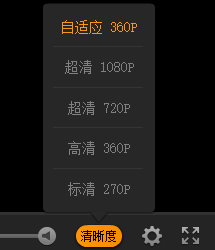
\includegraphics[height=1.9cm]{fig/bitrate_tencent.png}\hspace*{0.4cm}
	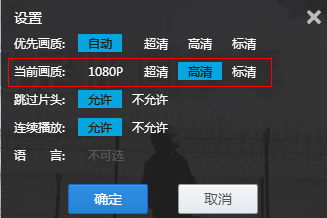
\includegraphics[height=1.9cm]{fig/bitrate_youku.png}\hspace*{0.4cm}
	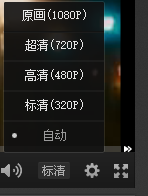
\includegraphics[height=1.9cm]{fig/bitrate_sohu.png}\hspace*{0.4cm}
	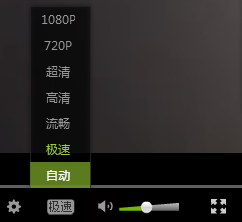
\includegraphics[height=1.9cm]{fig/bitrate_qiyi.png}   
\end{itemize}	
\end{frame}

\begin{frame}{Problems in traditional approaches for adaptive streaming} 
\begin{itemize}
	\item<1> only a small set of candidate bitrates to manually choose from\\ %
	cannot effectively adapt to the changing network conditions
	\item<1> huge computing resource consumption
	\begin{itemize}
		\item<1> coding to H.264: 1/3 to 2/3 of playback time
		\item<1> coding to H.265: 30+ times of playback time
		\item<1> one CPU core: only 1-2 concurrent coding tasks
	\end{itemize}
	\item<1> oblivious of users' \emph{preferences} of different \emph{peering servers}
\end{itemize}
\end{frame}

\section{Related Work}
\begin{frame}{DASH}
	Problems in HTTP Progressive Downloading. 
	\begin{itemize}
		\item<1> big media head $\longrightarrow$ long startup/VCR delay\\
		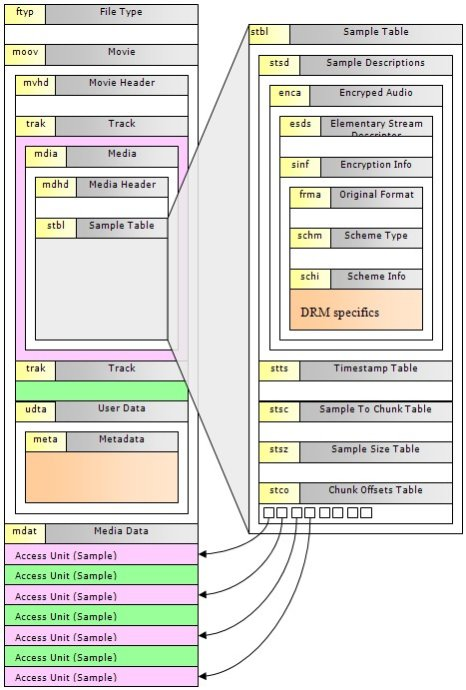
\includegraphics[height=4cm]{fig/MP4_boxes_detail.jpg}
		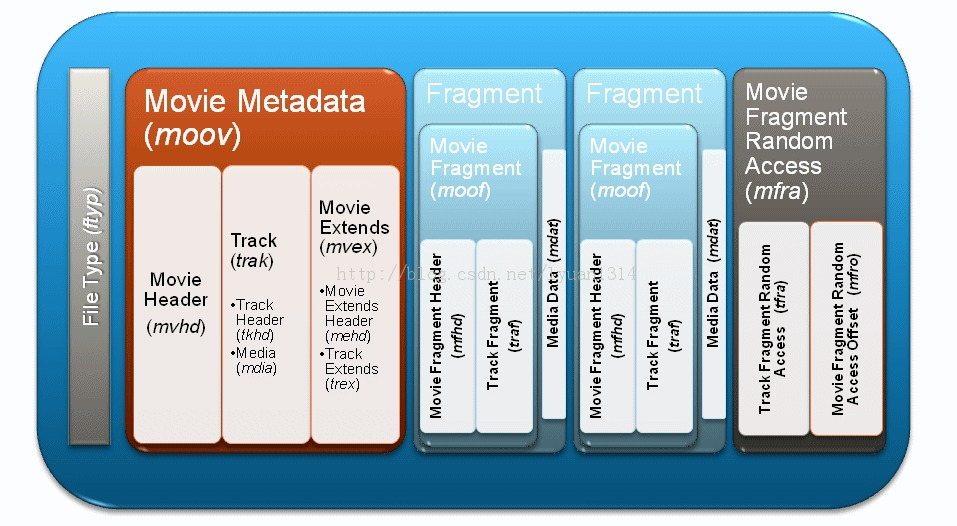
\includegraphics[height=4cm]{fig/fragmented_mp4.jpg}
	\end{itemize}
\end{frame}
\begin{frame}
	\begin{itemize}
		\item<1> 2nd time buffering due to varying download speed\\
		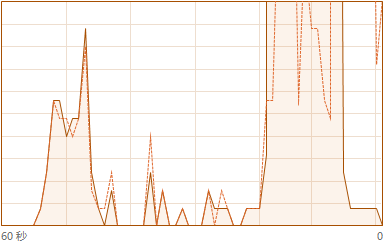
\includegraphics[height=5.4cm]{fig/download_speed.png}
	\end{itemize}
\end{frame}
\begin{frame}{DASH}
	DASH: Dynamic Adaptive Streaming over HTTP. \\
	Several industrial \& academic DASH standards: 
	\begin{itemize}
		\item<1> Apple HLS (HTTP Live Streaming) 2009
		\item<1> Microsoft HSS (HTTP Smooth Streaming) 2010
		\item<1> Adobe HDS (HTTP Dynamic Streaming) 2010
		\item<1> MPEG-DASH (ISO/IEC 23009-1) 2012
	\end{itemize}
\end{frame}
\begin{frame}{Working fashion of DASH: in a nutshell}
	\begin{center}
		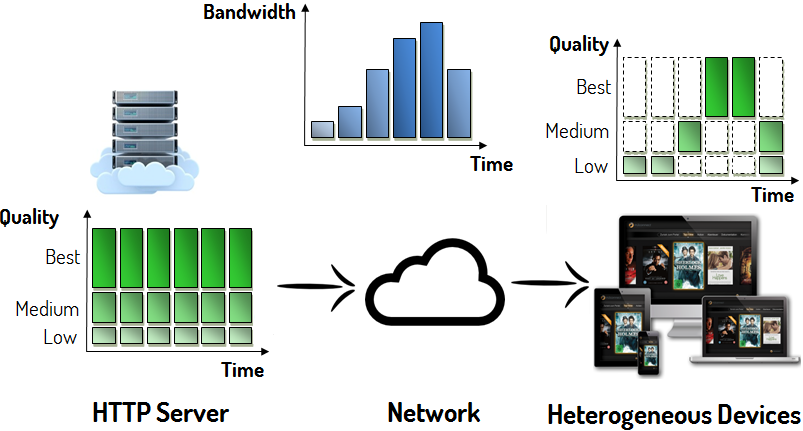
\includegraphics[height=6cm]{fig/adaptive-streaming.png}
	\end{center}
\end{frame}
\begin{frame}{Apple HLS}
	\begin{itemize}
		\item<1> Architecture
		\begin{center}
			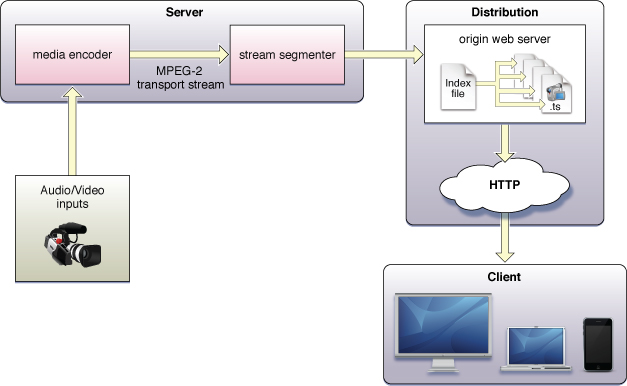
\includegraphics[height=4.5cm]{fig/hls_arch.jpg}
		\end{center}
	\end{itemize}
\end{frame}
\begin{frame}{Apple HLS}
	\begin{itemize}
		\item<1> Segment Indexing
		\begin{center}
			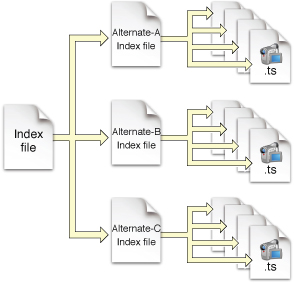
\includegraphics[height=4.5cm]{fig/hls_indexing.jpg}
		\end{center}
	\end{itemize}
\end{frame}

\begin{frame}{MPEG-DASH}
	\begin{itemize}
		\item<1> Architecture
		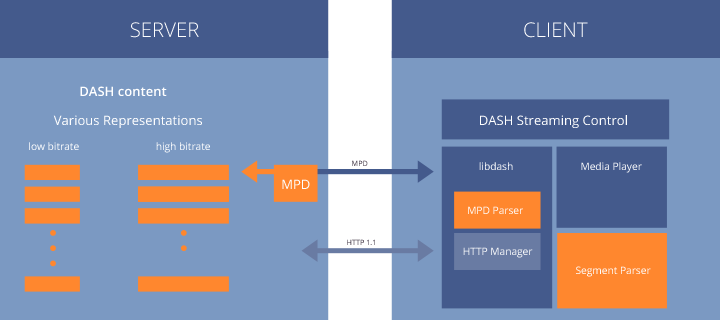
\includegraphics[height=4.5cm]{fig/MPEG-DASH_arch.png}
	\end{itemize}
\end{frame}
\begin{frame}{MPEG-DASH}
	\begin{itemize}
		\item<1> Data Model
		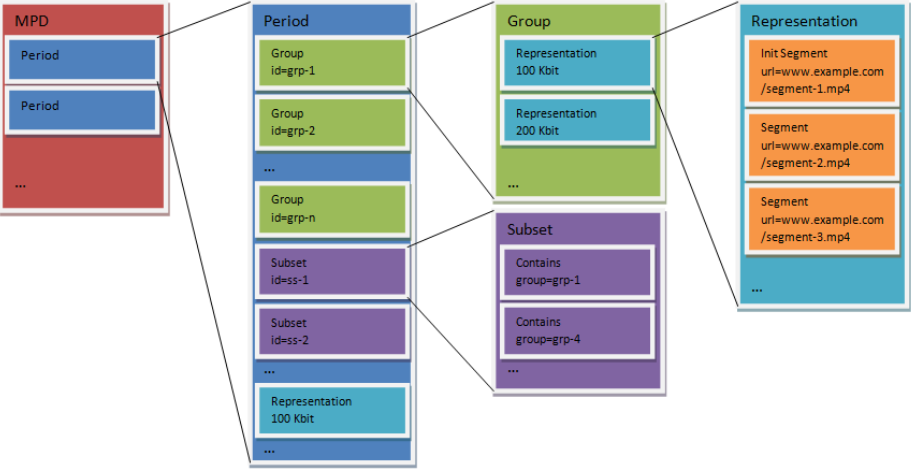
\includegraphics[height=4.5cm]{fig/mpeg-dash_data_model.png}
	\end{itemize}
\end{frame}
\begin{frame}{MPEG-DASH}
	\begin{itemize}
		\item<1> Segment Indexing
		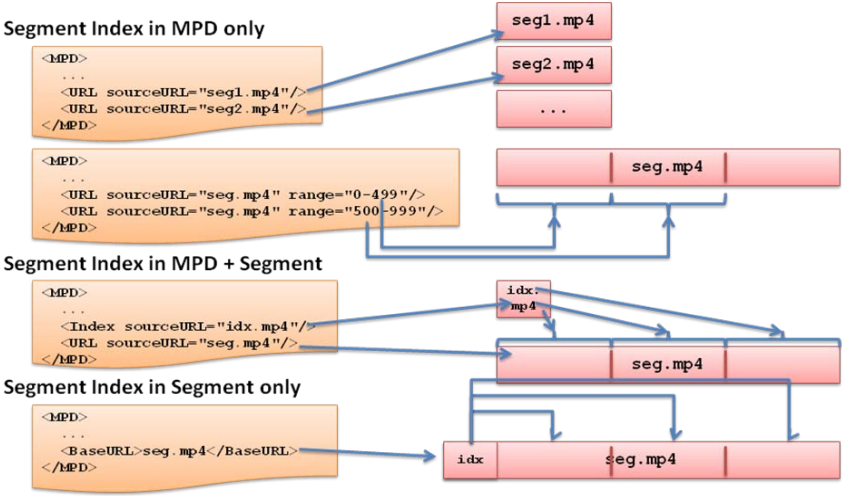
\includegraphics[height=5cm]{fig/mpeg-dash_indexing.png}
	\end{itemize}
\end{frame}

\begin{frame}{QoE in Streaming}
	\begin{itemize}
		\item<1> bitrate, packet loss, delay \\
		\bibentry{evalvid} \\
		\bibentry{wang2002image}
	\end{itemize}
\end{frame}
\begin{frame}{QoE in Streaming}
	\begin{itemize}
		\item<1> user activities also affect QoE in DASH\\
		\bibentry{Mok:2012:QQD:2155555.2155558}
		\item<1> no-reference metrics\\
		No-reference Video Quality: capture motion smoothness, motion artifacts, and spatial quality.
	\end{itemize}
\end{frame}

\begin{frame}{Streaming over CDNs}
	\begin{itemize}
		\item<1> traditional studies more focused on the network aspect\\
		improving the connectivity between streaming servers and users\\
		\bibentry{6195531}
	\end{itemize}
\end{frame}

\begin{frame}{Video Transcoding Schemes}
	\begin{itemize}
		\item<1> dedicated transcoders\\
		\bibentry{6195531}
		\item<1> SVC based\\
		\bibentry{5935009}
	\end{itemize}
\end{frame}
\begin{frame}{Video Transcoding Schemes}
	\begin{itemize}
		\item<1> MapReduce-based\\
		Alan Zhuang. Tencent TranscX. Cloud Transcoding System Reusing Idle Computational Resources on Storage Servers. CN201210490708.0; PCT/CN2013/085388.\\
		\bibentry{6271923}\\
		\item<1> previous transcoding paradigms\\
		doing media transcoding and media delivery separately
	\end{itemize}
\end{frame}

\section{Measurements \& Observations}
\begin{frame}{Video Viewing Patterns}
	\begin{itemize}
		\item<1> in BesTV (Professional Content)\\
		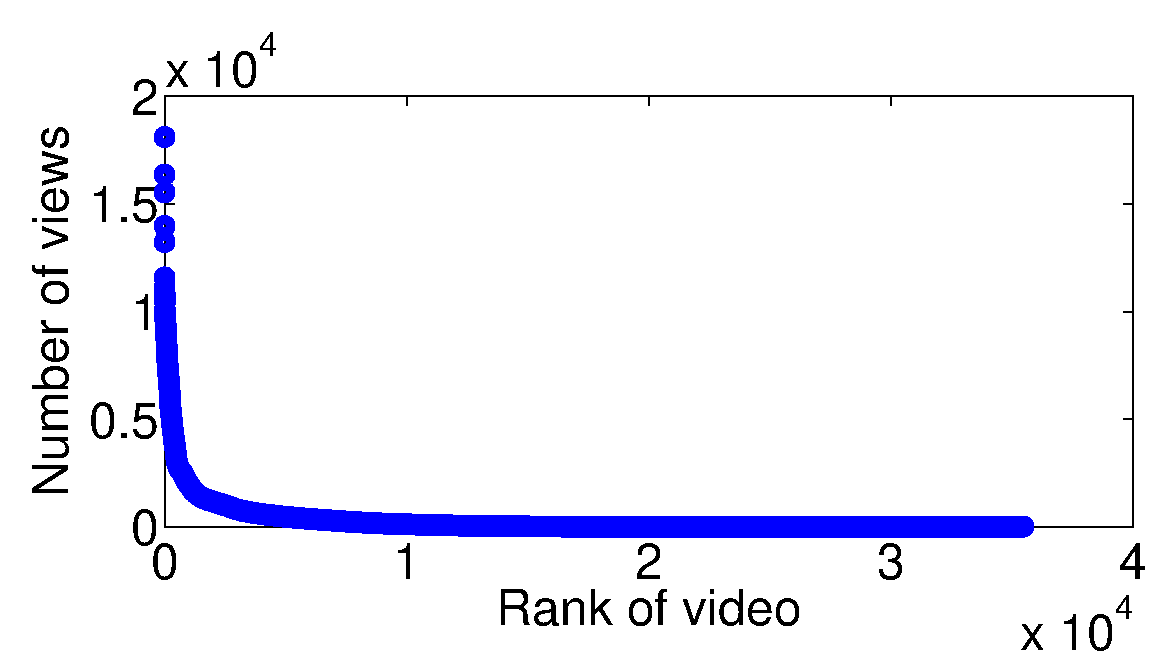
\includegraphics[height=2.2cm]{fig/video-freq.eps}
		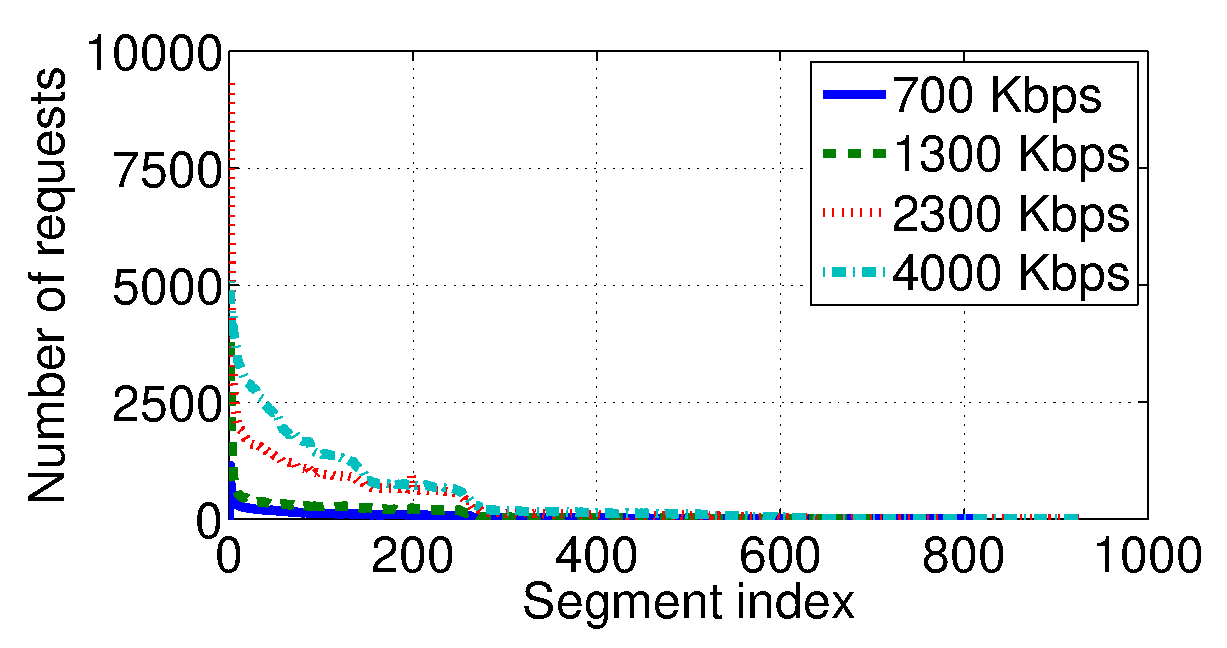
\includegraphics[height=2.2cm]{fig/sy-req-vs-seg.eps}
		\item<1> in WeiShi (UGC)\\
		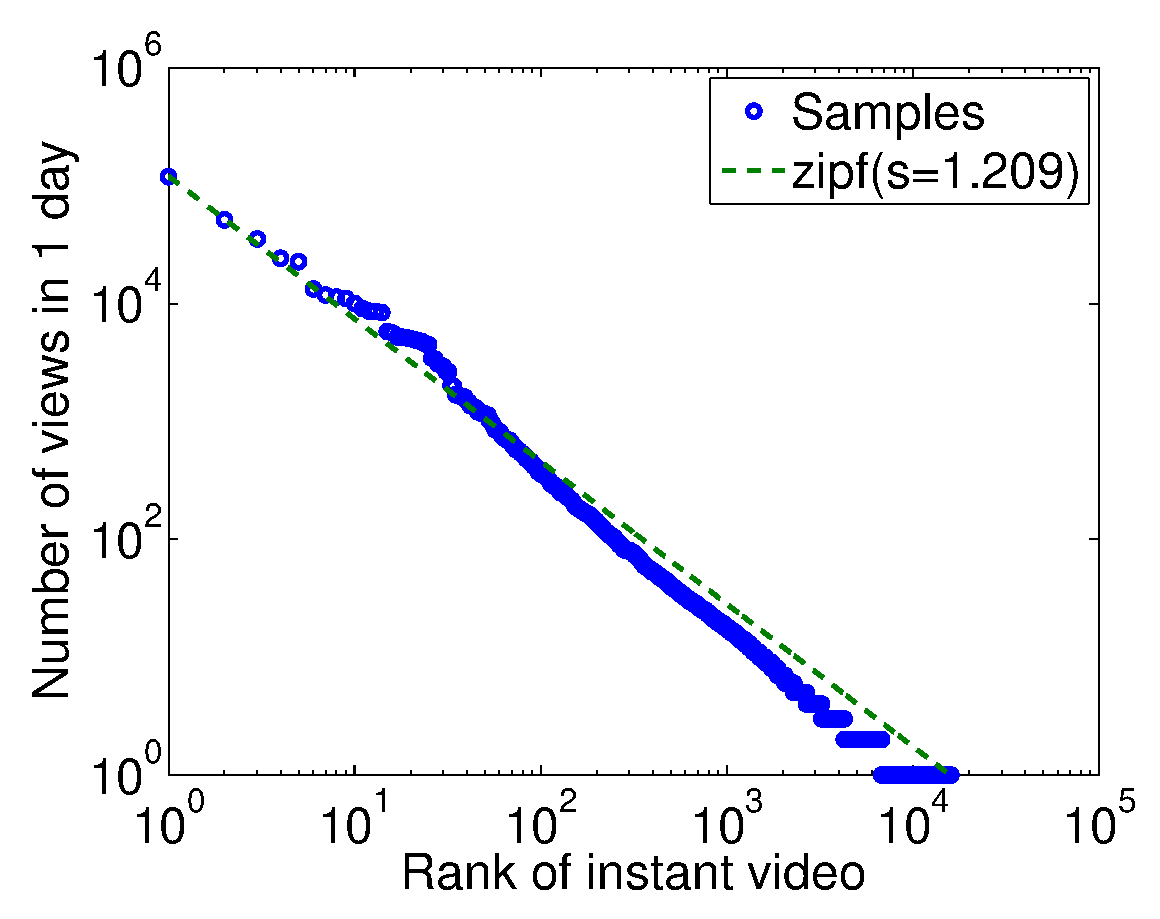
\includegraphics[height=2.1cm]{fig/video-popularity.eps}
		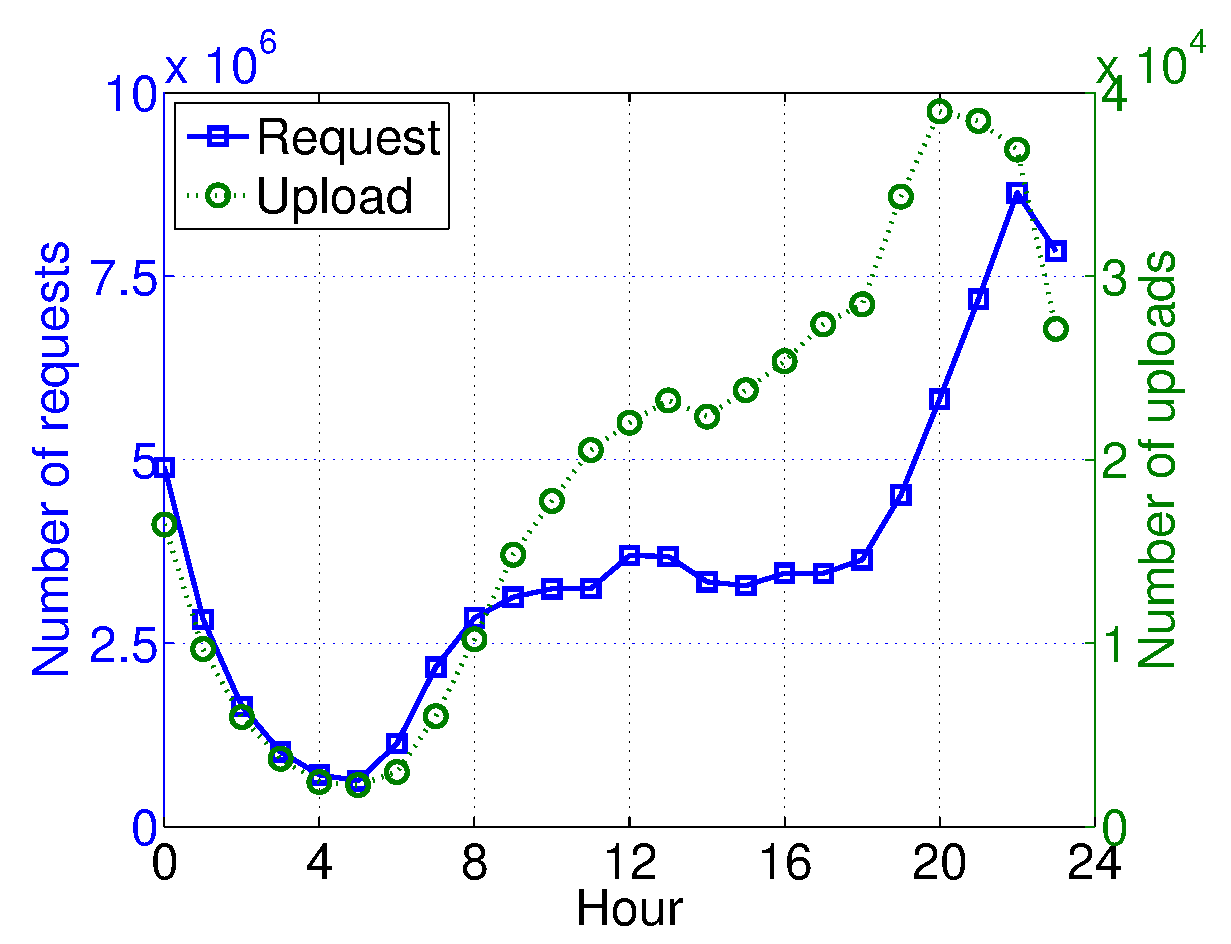
\includegraphics[height=2.1cm]{fig/request-upload-overtime.eps}
		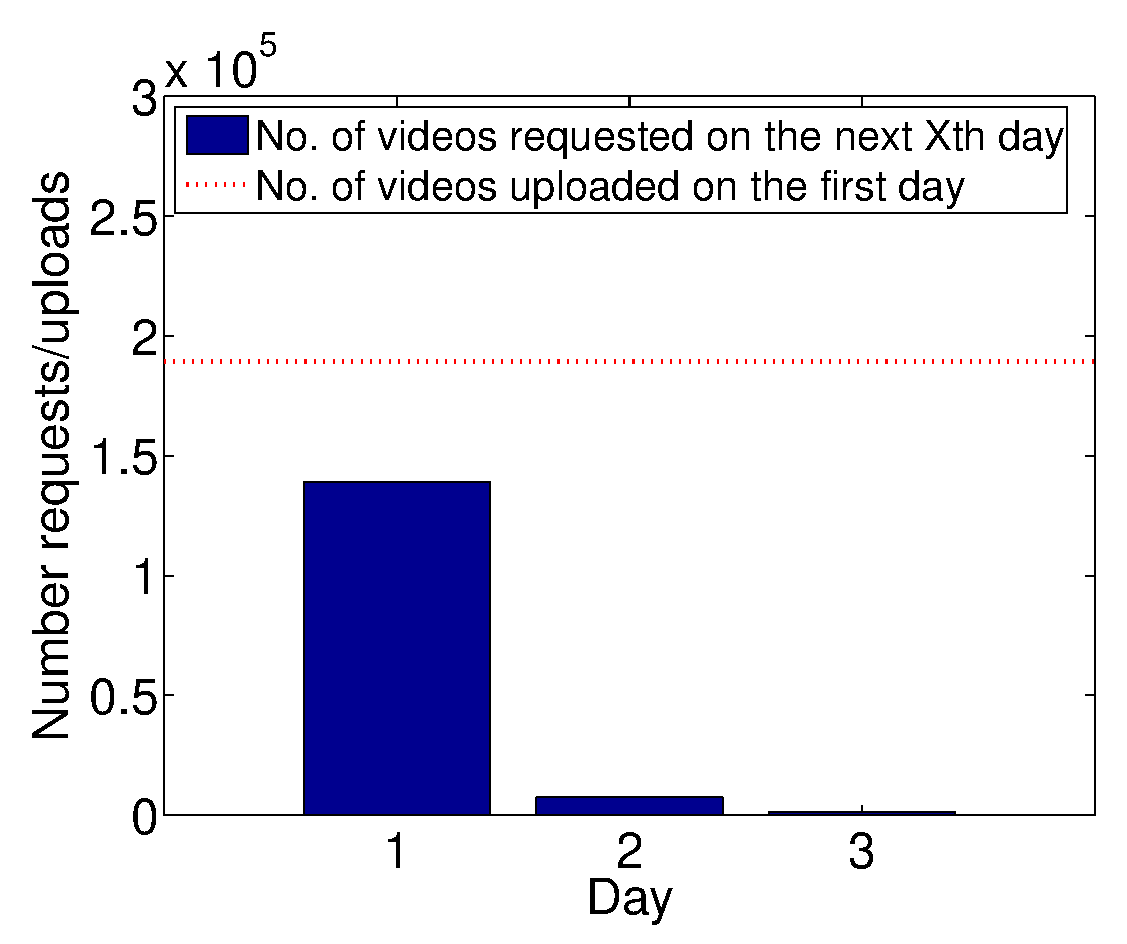
\includegraphics[height=2.1cm]{fig/view-in-3-days.eps}
		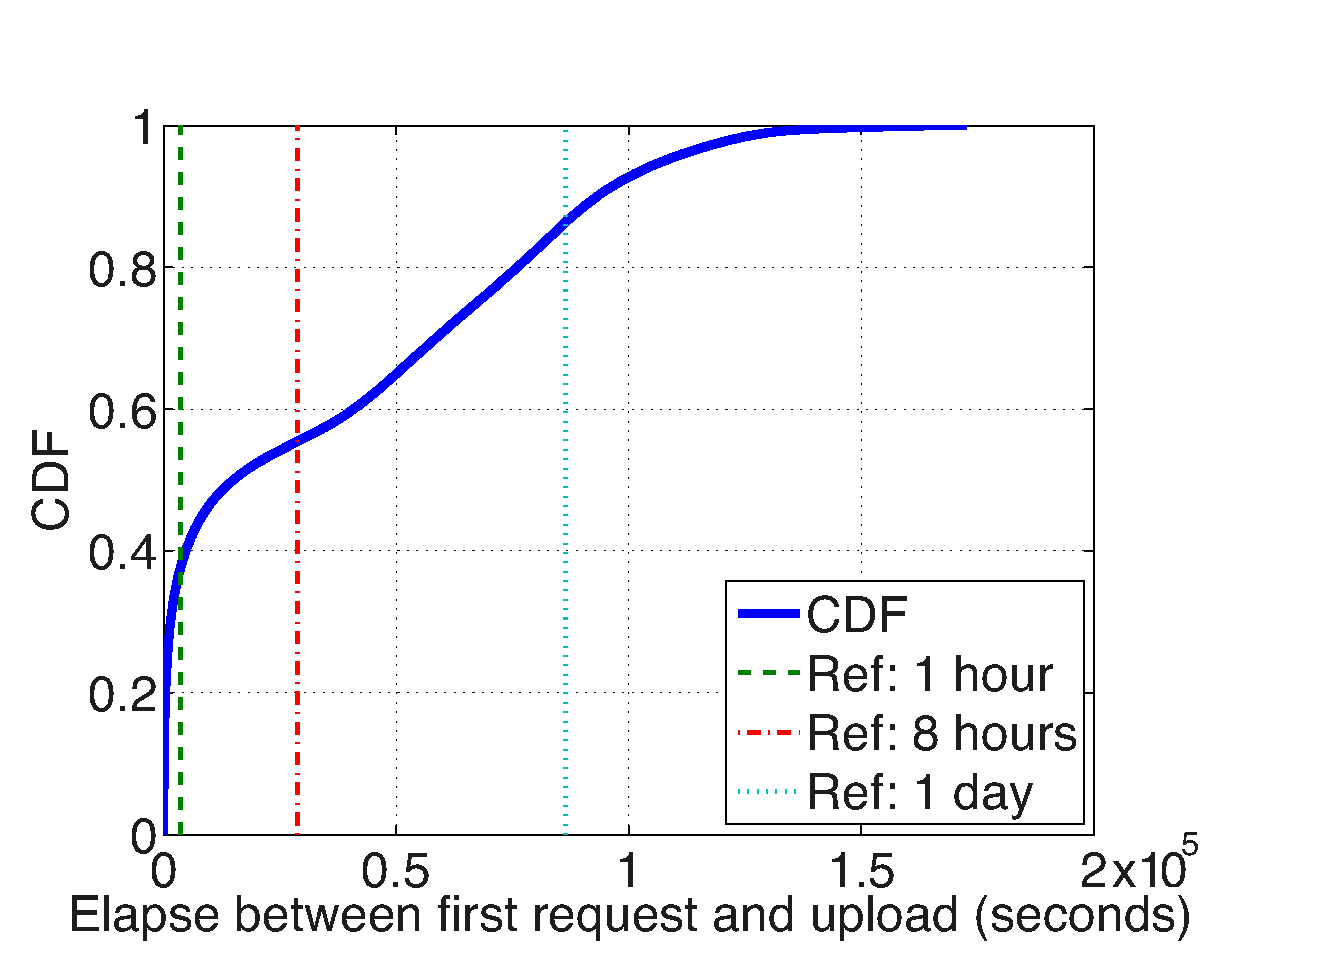
\includegraphics[height=2.2cm]{fig/updowntimediff.eps}
	\end{itemize}
\end{frame}

\begin{frame}{CDN Patterns}
	\begin{itemize}
		\item<1> CPU load patterns\\
		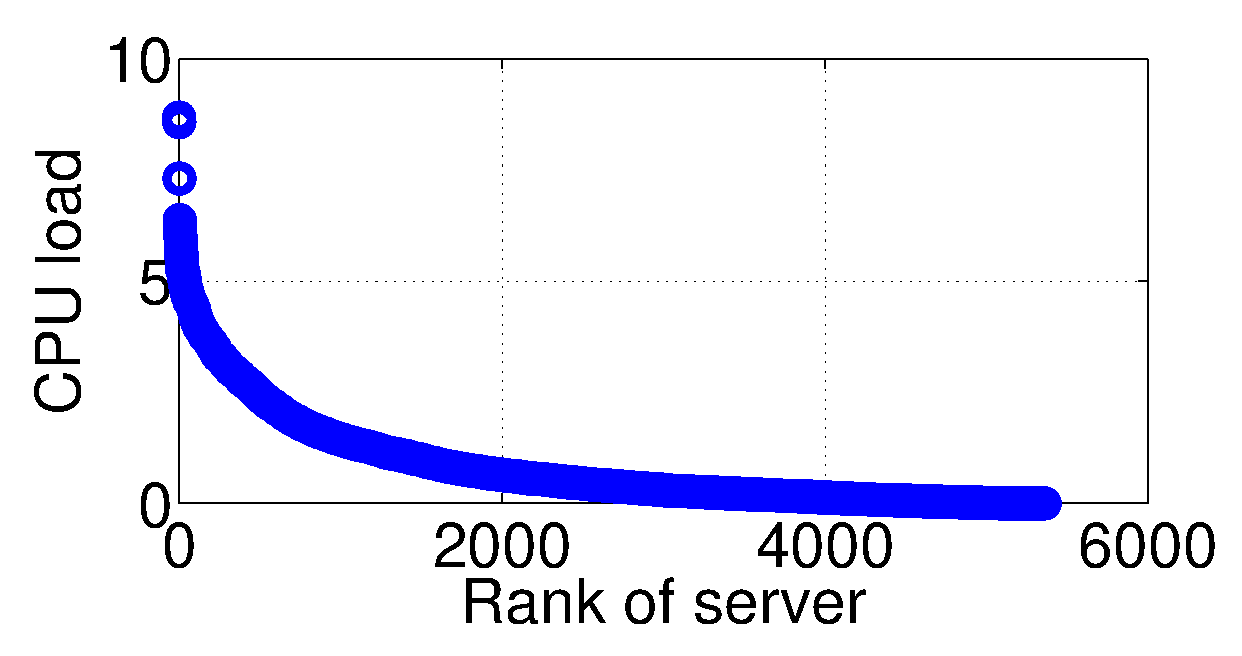
\includegraphics[width=0.27\linewidth]{fig/cpuload_vs_server.eps}
		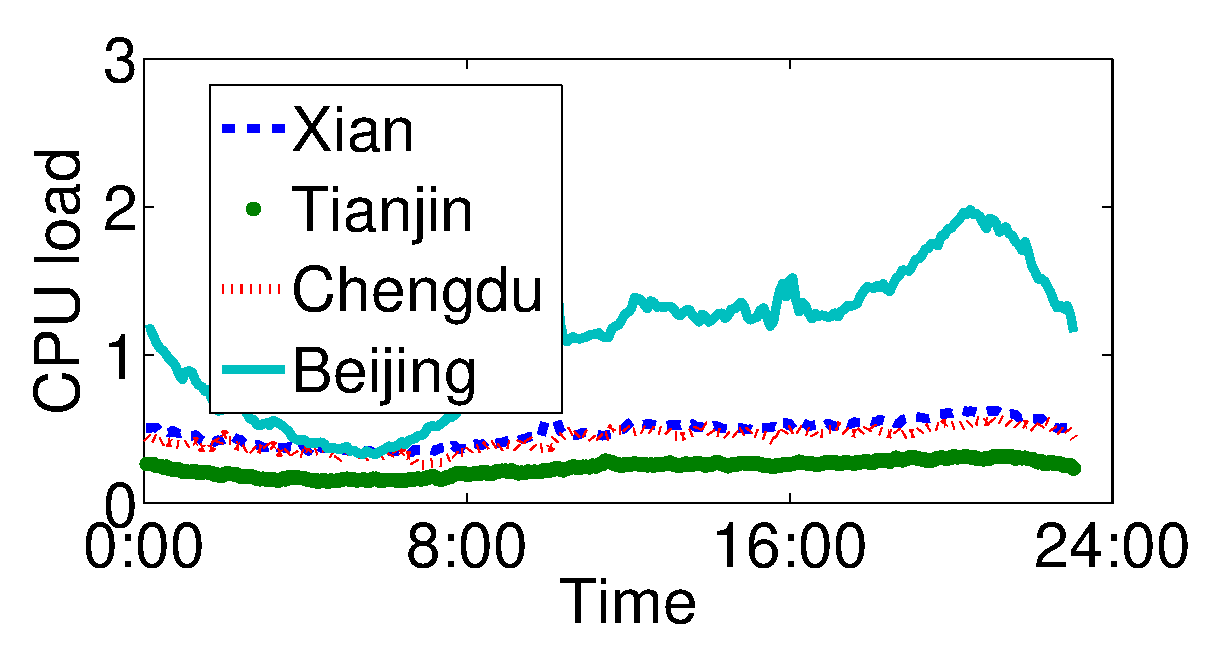
\includegraphics[width=0.26\linewidth]{fig/idc_cpuload_over_time.eps}
		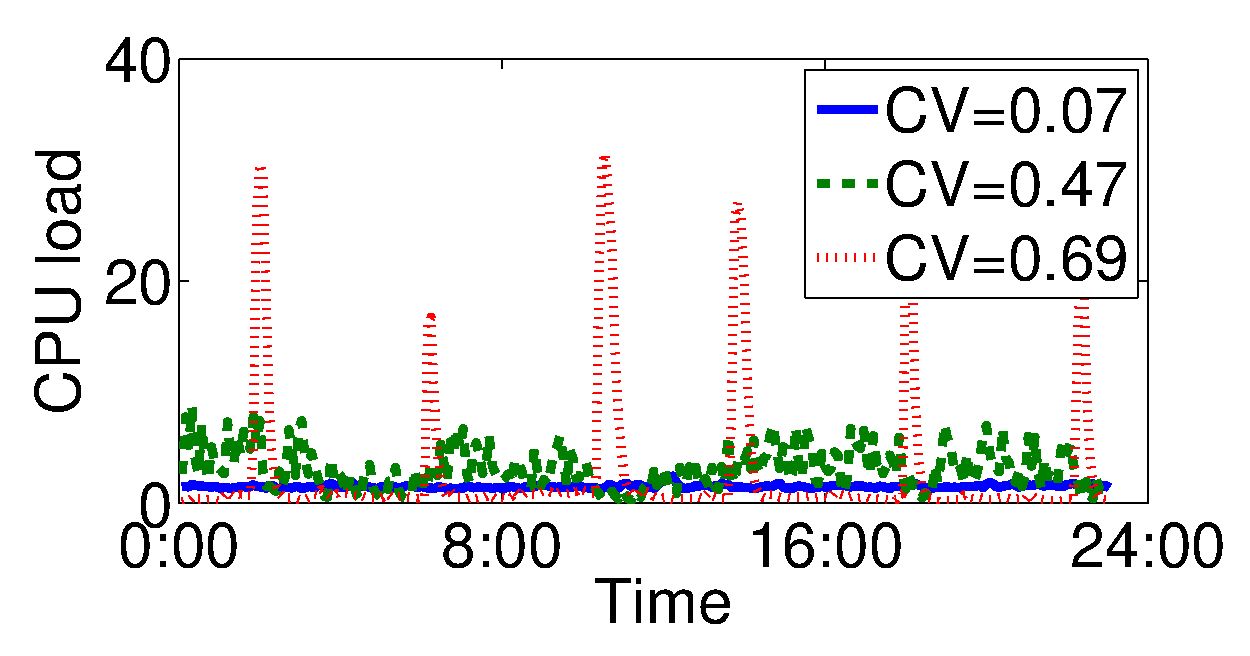
\includegraphics[width=0.27\linewidth]{fig/server_cpu_load_overtime.eps}
		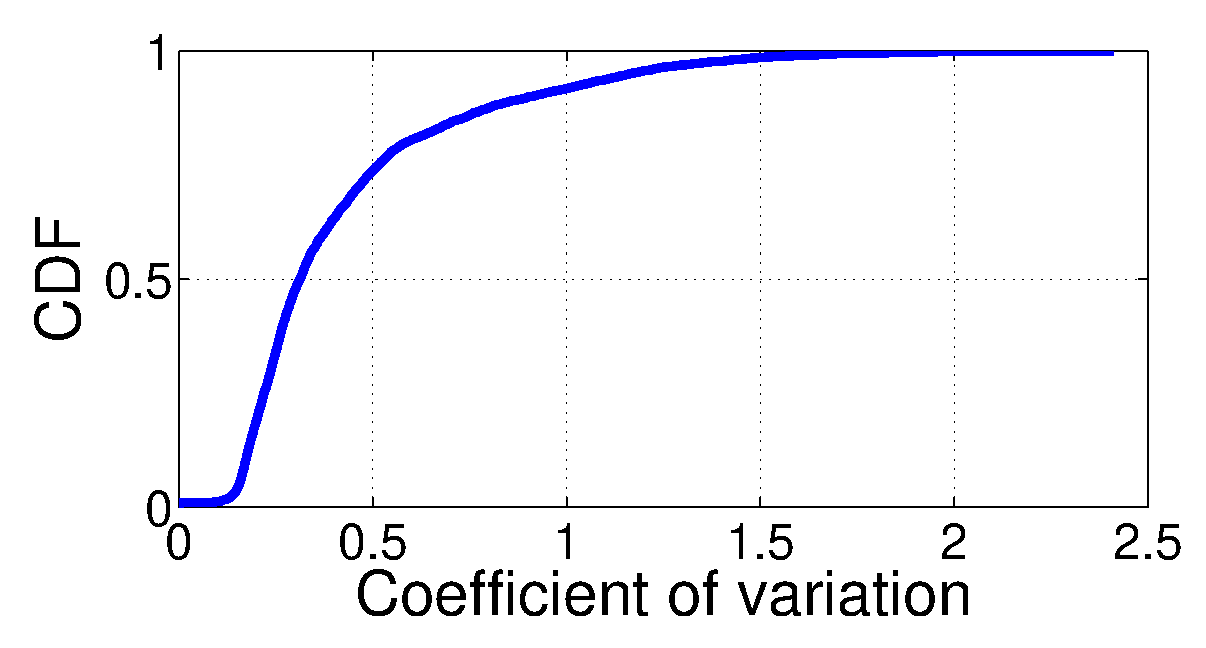
\includegraphics[width=0.26\linewidth]{fig/server_cv_cdf.eps}\footnote{$CV = 1/24 \sum_{h=0}^{23} {\sqrt{E[(X_h - \bar{X_h})^2]}}/{\bar{X_h}}$, $X_h$: CPU load in $h$}
		\item<1> bandwidth patterns\\
		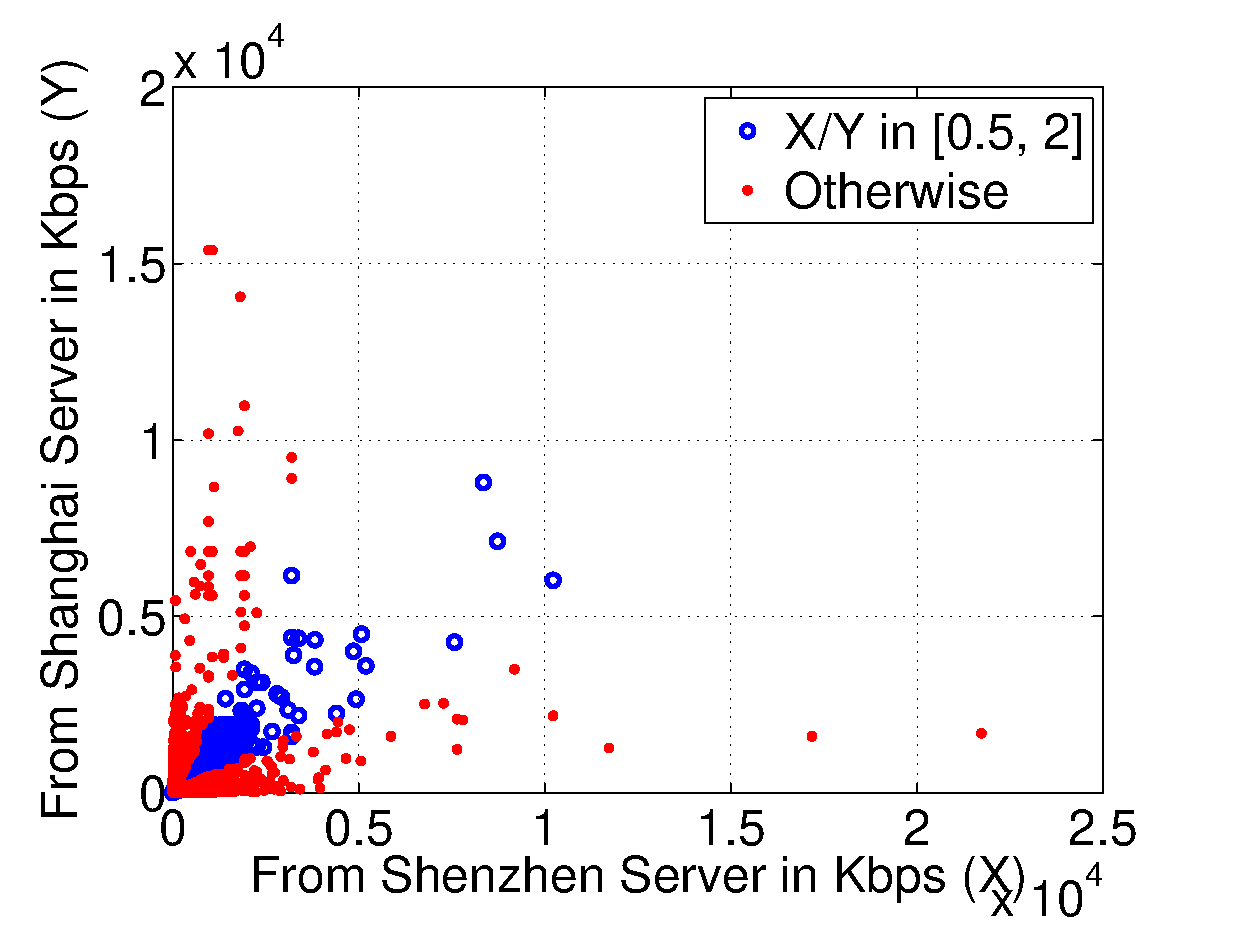
\includegraphics[width=0.27\linewidth]{fig/user-server-speed.eps}
		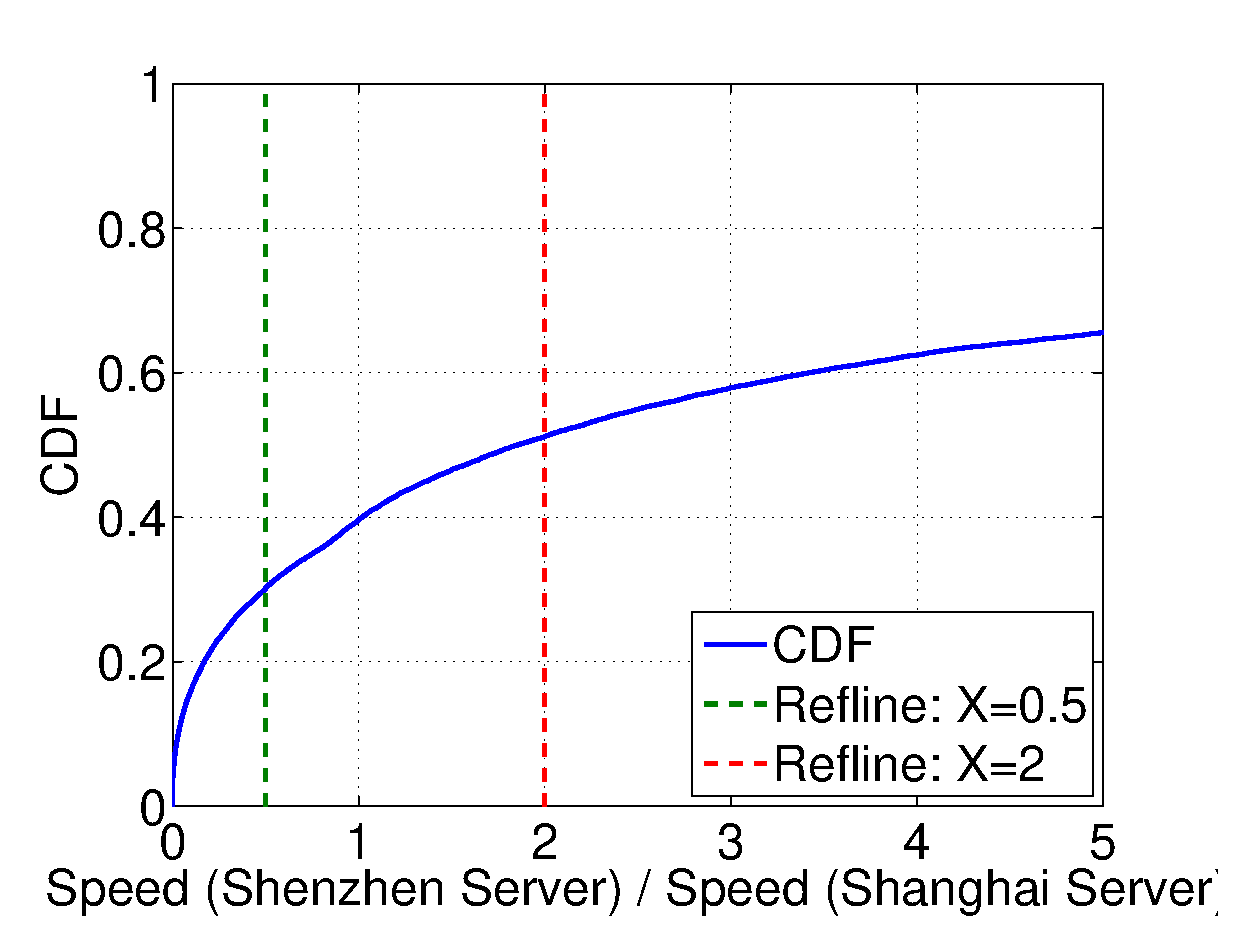
\includegraphics[width=0.27\linewidth]{fig/user-server-speed-ratio.eps}
		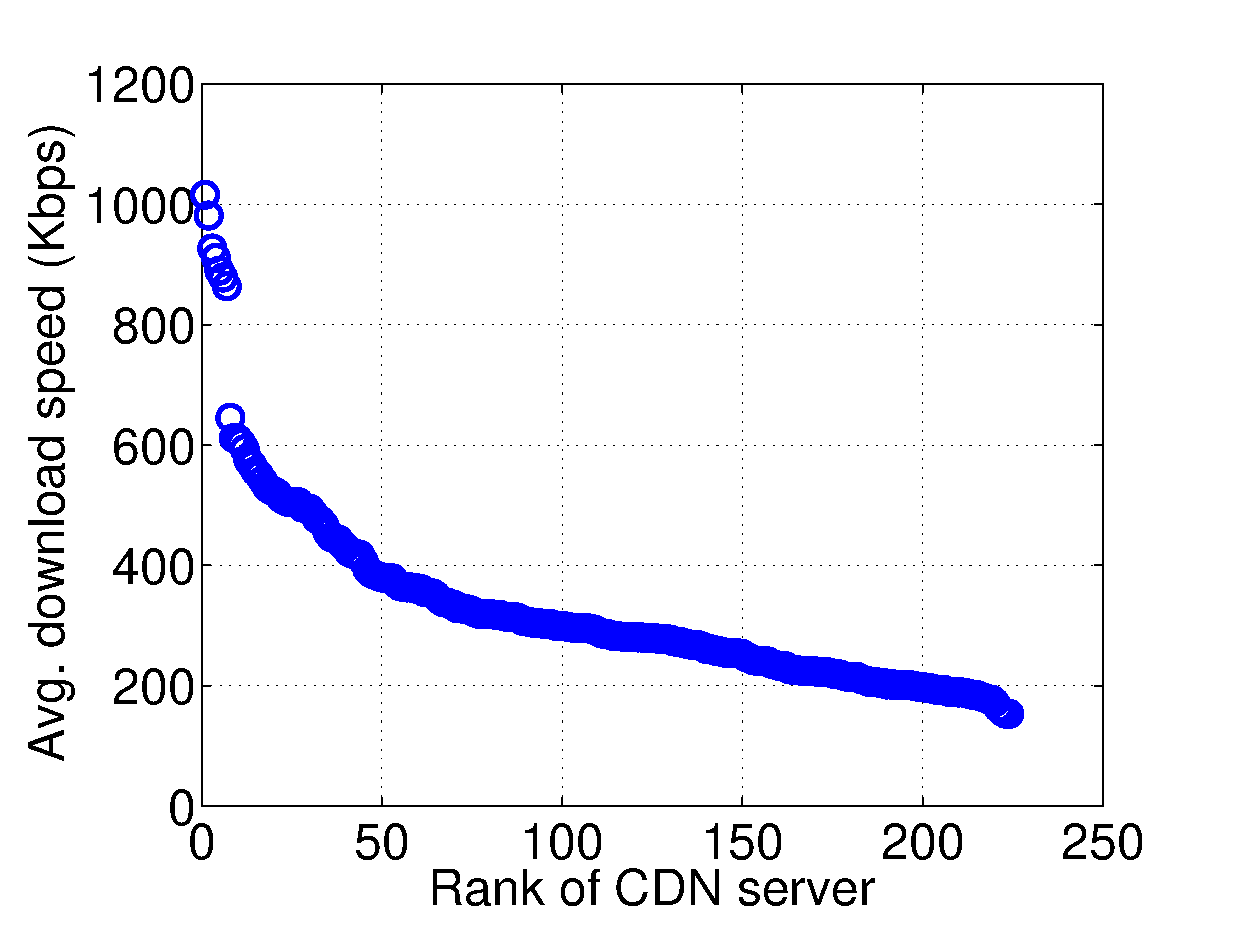
\includegraphics[width=0.27\linewidth]{fig/tencent_cdn_server_downloadspeed_20130504.eps}
		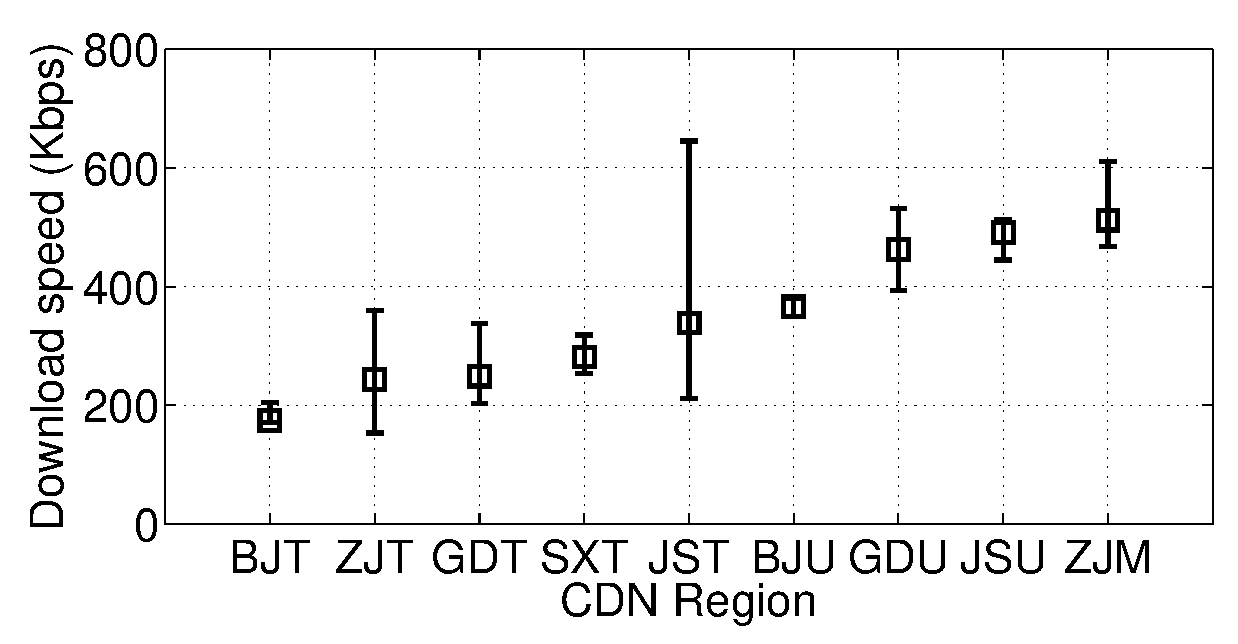
\includegraphics[width=0.27\linewidth]{fig/region-speed-distribution.eps}
	\end{itemize}
\end{frame}

\begin{frame}{CDN Patterns: a long-term view}
	\begin{itemize}
		\item<1> total bandwidth of a CDN region of Tencent CDN\\
			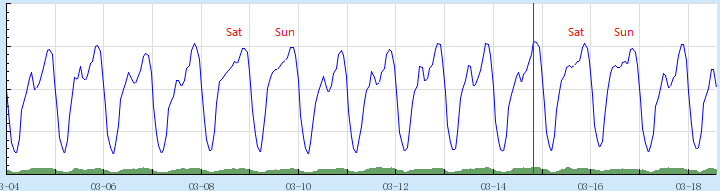
\includegraphics[width=0.7\linewidth]{fig/bandwidth.png}
		\item<1> CPU utilization of a server in this region\\
			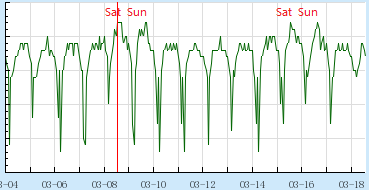
\includegraphics[width=0.7\linewidth]{fig/cpu_utilization.png}	
	\end{itemize}
\end{frame}

\begin{frame}{Insights}
	\begin{itemize}
		\item<1> pre-transcoding all to all versions is unnecessary\\
		pre-transcoding every segment of all videos to an increasing number of versions is a huge waste of computing resource
		\item<1> most backend servers in CDNs are predictably(stably) idle\\
		thus can be scheduled for transcoding
		\item<1> users have preferences towards CDN regions\\
		\item<1> regions have preferences towards media versions\\
	\end{itemize}
\end{frame}

\section{Joint Transcoding \& Delivery}

\begin{frame}{Joint Online Transcoding and GeoISP-Distributed Delivery}
	Framework: (in terms of time-slots)
	\begin{itemize}
		\item<1> rank users' preferences towards different CDN regions\\
		available bandwidth estimation e.g. \emph{abget}, for rank of download speeds
		\item<1> predict number of requests for a particular segment\\
		assume mostly in a consecutive way, issuing few VCR operations
		\item<1> predict idle computing resource\\
		just use the status of the last slot, or LR, ARIMA, ANN, ...
	\end{itemize}
	\begin{center}
	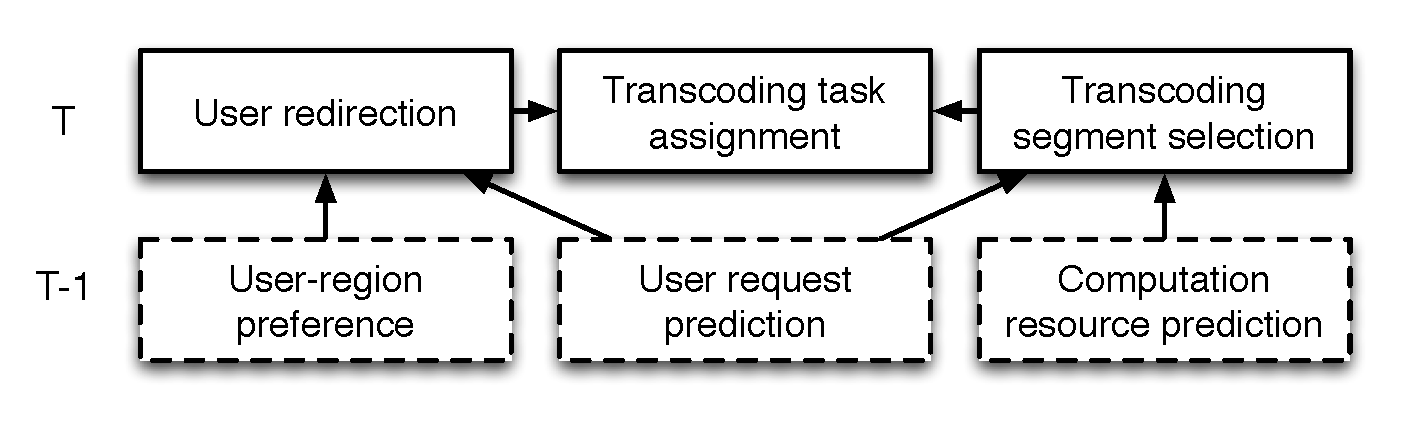
\includegraphics[width=0.7\linewidth]{fig/framework.eps}
	\end{center}
\end{frame}

\begin{frame}{Joint Online Transcoding and GeoISP-Distributed Delivery}
	Architecture:
	\begin{center}
		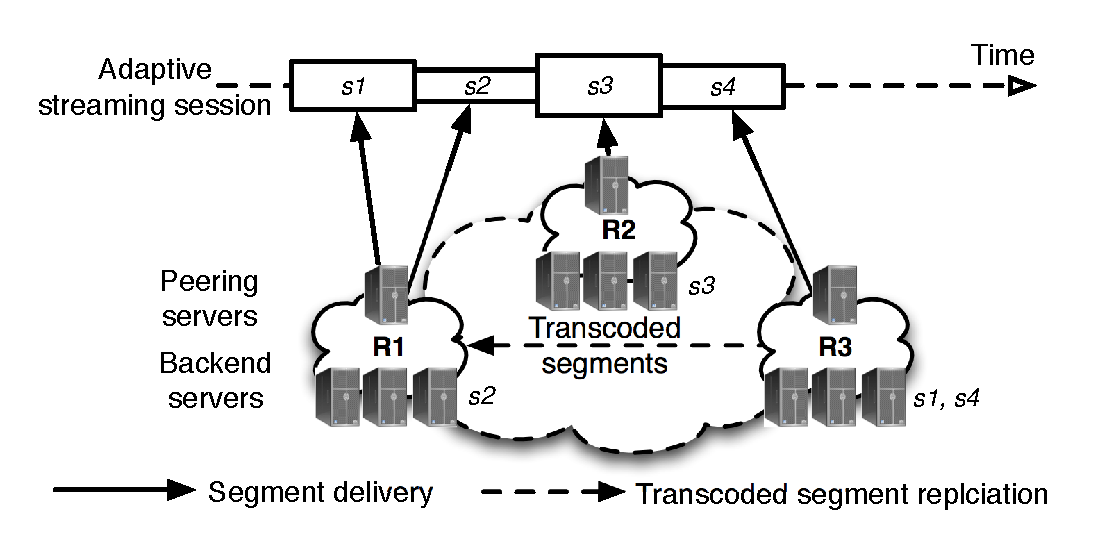
\includegraphics[width=\linewidth]{fig/geo-on-demand.eps}
	\end{center}
\end{frame}

\begin{frame}{Joint Online Transcoding and GeoISP-Distributed Delivery}
	Architecture: Girls Chasing Boys?
	\begin{center}
		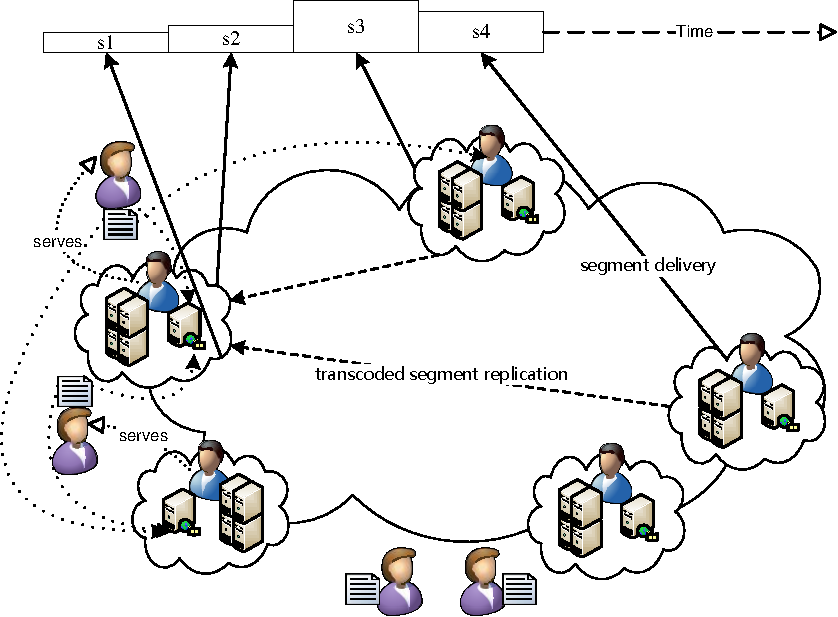
\includegraphics[width=0.8\linewidth]{fig/transcoding_delivery.pdf}
	\end{center}
\end{frame}

\begin{frame}{Joint Online Transcoding and GeoISP-Distributed Delivery}
	Mechanism:
	\begin{itemize}
		\item<1> user request redirection\\
		to her ideal CDN region, and then do a load-balancing e.g. round-robin
		\item<1> transcoding segment selection\\
		using backend servers with idle computing resource, in terms of closed GoPs that can be transcoded independently;\\
		if cannot be transcoded timely, send a closest lower alternative bitrate version 
		\item<1> transcoding task assignment\\
		transcoding is performed in selected regions;\\
		transcoded segments will be cached by the backend servers and replicated to other regions;\\
		replication cost should be minimized		
	\end{itemize}
\end{frame}

\begin{frame}{QoE-Driven Redirection: Notations}
	\centering
	\begin{tabular}{|p{0.15\linewidth}||p{0.75\linewidth}|}
		\hline 
		Symbol & Definition \\ 
		\hline
		\emph{$\Users^{(T)}$} 		& Set of users requesting segments in time slot $T$ \\
		\emph{$\CDNRegions$} 		& Set of CDN regions  \\
		\emph{$\Redirect^{(T)}_{u,r}$} 		& Binary variable indicating whether user $u$ will download from region $r$ in time slot $T$\\
		\emph{$\USPref_{u,r}$} 		& Preference level for user $u$ to receive video stream from region $r$ \\ 
		\emph{$\bandwidth_r$} 		& Bandwidth capacity of  region $r$ \\ 	
		\emph{$\Bitrate_v$} 		&  Bitrate of a particular version $v$ \\
		\emph{$\Version_{u,r}$} 		&  Highest version that $u$ can receive when she downloads from region $r$ \\
		\hline 
	\end{tabular} 
\end{frame}

\begin{frame}{QoE-Driven Redirection: Problem Formulation}
	\begin{equation}
	\max_{\Redirect^{(T)}} \sum_{u \in \Users^{(T)}, r \in \CDNRegions} \USPref_{u,r} \Redirect^{(T)}_{u,r},
	\label{eq:redirect}
	\end{equation}
	subject to:
	\[
	\begin{split}
	\sum_{r \in \CDNRegions} \Redirect^{(T)}_{u,r} & \le 1, \forall u \in \Users^{(T)},\\	
	\sum_{u \in \Users^{(T)}} \Redirect^{(T)}_{u,r} \Bitrate_{\Version_{u,r}} & \le \bandwidth_{r}, \forall r \in \CDNRegions,\\
	\Redirect^{(T)}_{u,r} & \in \{0,1\}, \forall u \in \Users^{(T)}, r \in \CDNRegions,
	\end{split}
	\]
\end{frame}

\begin{frame}{QoE-Driven Redirection: NP-hardness Proof}
	\begin{theorem}
		Redirecting users to CDN regions such that their preferences can be maximally satisfied, as formulated in (\ref{eq:redirect}), is NP-hard.
	\end{theorem}
	
	\begin{proof}
		Reduce a conventional 0/1 knapsack to this problem:
		$$
		\max \sum_{i=1}^{n}v_i x_i,
		$$
		subject to
		$$
		\sum_{i=1}^{n} \alpha_i x_i \le \beta, 
		x_i \in \{0,1\},
		$$
	\end{proof}
\end{frame}	

\begin{frame}{QoE-Driven Redirection: NP-hardness Proof}
	\begin{proof}
	\begin{enumerate}
		\item<1> Let $\Users^{(T)} = \{1,2,\ldots,n\}$, $\CDNRegions=\{1\}$;
		\item<1> Let $\USPref_{i,1} = v_i, i = 1,2,\dots,n$;
		\item<1> Let $\Bitrate_{\Version_{i,1}} = \alpha_i, i=1,2,\ldots,n$;
		\item<1> Let $\bandwidth_1 = \beta$.
	\end{enumerate}
	The reduction operations take linear time, and the final results for the 0/1 knapsack problem are $x_i = \Redirect^{(T)}_{i,1}, i=1,2,\dots,n$. Therefore, our problem is NP-hard. 
	%\alt<3>{\qedhere}{\phantom\qedhere}
	\end{proof}
\end{frame}

\begin{frame}{QoE-Driven Redirection: Our Heuristic Algorithm}
	\begin{enumerate}
		\item<1> Bootstrap\\
		When a user requests to watch a video, assign her a list of candidate peering servers from regions with the lowest load.
		\item<1> Users rank servers\\
		in descending order of the estimated download speeds, and send connection requests to these servers.
		\item<1> Servers rank users\\
		only accept a portion of users according to its available bandwidth $\bandwidth_r$. The request from user $u$ is prioritized to be accepted if she has a larger $\USPref_{u,r}/\Bitrate_{\Version_{u,r}}$ with the CDN region $r$. 
		\item<1> Users finally decide\\
		A user selects the best peering server from the ones accepting her request according to the ranked list.
	\end{enumerate}
\end{frame}

\begin{frame}{QoE-Driven Redirection: Essentially...}
	\begin{itemize}
		\item<1> Like a Stable Matching\\
		but simplified.
		\item<1> More Boston-like\\
		rather than a DA(Deferred Acceptance) fashion.
		\item<1> Easy to be implemented\\
		and executed.
		\item<1> Works efficiently\\
		 in real-world in distributed manner!
	\end{itemize}
\end{frame}

\begin{frame}{Prioritizing Sgement Transcoding Tasks: Notations}
	\centering
	\begin{tabular}{|p{0.10\linewidth}||p{0.89\linewidth}|}
		\hline 
		Symbol & Definition \\ 
		\hline
		\emph{$\RequestingSeg^{(T)}$} 		& The set of segments being requested in time slot $T$ \\ 
		\emph{$\TranscodeIndicator^{(T)}_{(s,v)}$} 		& Indicator: if segment $(s,v)$ will be transcoded \\ 
		\emph{$e_{(s,v)}^{(T)}$} 		& Importance level of a particular segment $(s,v)$ in $T$  \\
		\emph{$\ReqOfSeg^{(T)}_{(s,v)}$} 		& Number of requests of segment $(s,v)$  from all regions in $T$ \\
		\emph{$\SegQuality_{(s,v)}^{(T)}$} 		& Quality gain if segment $(s,v)$ is transcoded in $T$\\
		\emph{$\Bitrate_v$} 		&  Bitrate of a particular version $v$ \\
		\emph{$\Version_{u,r}$} 		&  Highest version $u$ can receive when downloads from region $r$ \\
		\emph{$\setS^{(T)}_{s}$} 		& The set of transcoded versions of segment $s$  \\
		\emph{$\comp_{(s,v)}$} 		& Computing resource required to perform the transcoding task to generate a segment $s$ of version $v$ \\
		\emph{$\IdleComp^{(T)}_r$} 		& Available computing resource that can be allocated for video transcoding from region $r$ in $T$ \\
		\hline 
	\end{tabular} 
\end{frame}

\begin{frame}{Prioritizing Sgement Transcoding Tasks: Formulation}
	$$e_{(s,v)}^{(T)} = \ReqOfSeg^{(T)}_{(s,v)} \SegQuality_{(s,v)}^{(T)},$$
	$$
	\SegQuality_{s,v}^{(T)} = \begin{cases}
	\min_w(\Bitrate_{v} - \Bitrate_{w})/{\Bitrate_{v}}, & \exists w \in \setS^{(T)}_s, w < v \\
	1, & \text{otherwise}
	\end{cases}.
	$$
	Problem:
	\begin{equation}
	\max_{\TranscodeIndicator^{(T)}} \sum_{(s,v) \in \RequestingSeg^{(T)}} \TranscodeIndicator^{(T)}_{(s,v)} e_{(s,v)}^{(T)}, 
	\end{equation}
	subject to:
	\[
	\begin{split}
	\sum_{(s,v) \in \RequestingSeg^{(T)}} \TranscodeIndicator^{(T)}_{(s,v)} \comp_{(s,v)} & \le \sum_r \IdleComp^{(T)}_r, \\
	\TranscodeIndicator^{(T)}_{(s,v)} & \in \{0,1\}, \forall (s,v) \in \RequestingSeg^{(T)}, \\
	\end{split}
	\]
\end{frame}

\begin{frame}{Prioritizing Sgement Transcoding Tasks: Solution}
	It is a 0-1 knapsack problem.
	\begin{enumerate}
		\item<1> Predicting\\
		Collect the information for prediction in a centralized manner, \emph{e.g.}, users (\emph{resp.} backend servers) report which segments they are downloading (\emph{resp.} the CPU load information) to a centralized server.
		\item<1> Ranking\\
		Based on the prediction, rank the requested segments in descending order of $e_{(s,v)}^{(T)}/\comp_{(s,v)}$.
		\item<1> Selecting\\
		Iteratively select segments from the ranked list to transcode, and update computation resource consumption, until the available idle computing resource is used up.
	\end{enumerate}
\end{frame}

\begin{frame}{Scheduling Transcoding Tasks across Regions: Notations}
	\centering
	\begin{tabular}{|p{0.13\linewidth}||p{0.84\linewidth}|}
		\hline 
		Symbol & Definition \\ 
		\hline
		\emph{$\CDNRegions$} 		& Set of CDN regions  \\
		\emph{$\TranscodeSet^{(T)}$} 		& Set of segments to be transcoded in time slot $T$  \\
		\emph{$\comp_{(s,v)}$} 		& Computation resource required to perform the transcoding task to generate a segment $s$ of version $v$ \\
		\emph{$\IdleComp^{(T)}_r$} 		& Available computation resource that can be allocated for video transcoding from region $r$ in $T$ \\
		\emph{$\SegRepCost_{(s,v),r}$} 		& Overall replication cost when segment $(s,v)$ is transcoded in region $r$ \\
		\emph{$\Assign^{(T)}_{(s,v),r}$} 		& Indicator: whether $(s,v)$ is transcoded in region $r$ in $T$ \\
		\emph{$\ReqFromRegion^{(T)}_{(s,v),r'}$} & Number of requests of $(s,v)$ to be served by a region $r'$ \\
		\emph{$\RegionRepCost_{r,r'}(s,v)$} & Replication cost when $(s,v)$ is replicated from $r$ to $r'$\\
		\hline 
	\end{tabular} 
\end{frame}

\begin{frame}{Scheduling Transcoding Tasks across Regions: Formulation}
	$$
	\SegRepCost_{(s,v),r} = \sum_{r' \ne r, \ReqFromRegion^{(T)}_{(s,v),r'} > \beta} \RegionRepCost_{r,r'}(s,v),
	$$
	Problem:
	\begin{equation}
	\min_{\Assign^{(T)}} \sum_{(s,v) \in \TranscodeSet^{(T)}} \sum_{r \in \CDNRegions} \Assign^{(T)}_{(s,v),r} \SegRepCost_{(s,v), r},
	\end{equation}
	subject to:
	\[
	\begin{split}
	\Assign^{(T)}_{(s,v),r} & \in \{0,1\}, \forall (s,v) \in \TranscodeSet^{(T)}, r \in \CDNRegions \\
	\sum_{r \in \CDNRegions} \Assign^{(T)}_{(s,v),r} &= 1, \forall (s,v) \in \TranscodeSet^{(T)}\\
	\sum_{(s,v) \in \TranscodeSet^{(T)}} \Assign^{(T)}_{(s,v),r} \comp_{(s,v)} & \le \IdleComp^{(T)}_r, \forall r \in \CDNRegions.
	\end{split}
	\]
\end{frame}

\renewcommand{\thealgorithm}{}

\begin{frame}[fragile]{Scheduling Transcoding Tasks across Regions: Solution}
	\begin{algorithm}[H]
		\caption{Transcoding task schedule.}\label{alg:transcoding-task-schedule}
		%\Procedure{Transcoding Task Schedule}{} 
		\begin{algorithmic}[H]	
			\STATE Let $M_{r} = \IdleComp^{(T)}_r, r \in \CDNRegions$
			\STATE Let $\Assign^{(T)}_{(s,v),r} = 0, \forall (s,v) \in \TranscodeSet^{(T)}, r \in \CDNRegions$
			\STATE Rank CDN region and segment pairs ($r-(s,v)$) in ascending order of $\SegRepCost_{(s,v),r}$
			\FOR{$\forall r-(s,v)$ in the ranked list}
			\IF{$\comp_{(s,v)} \le M_r$}
			\STATE Let $M_r = M_r - \comp_{(s,v)}$
			\STATE Let $\Assign^{(T)}_{(s,v),r} = 1$
			\STATE Remove pairs with $(s,v)$ from the ranked list
			\ENDIF
			\ENDFOR
		%\EndProcedure
		\end{algorithmic}
	\end{algorithm}
\end{frame}

\begin{frame}{Effects}
	\begin{itemize}
		\item<1> Computing resource saved\\
			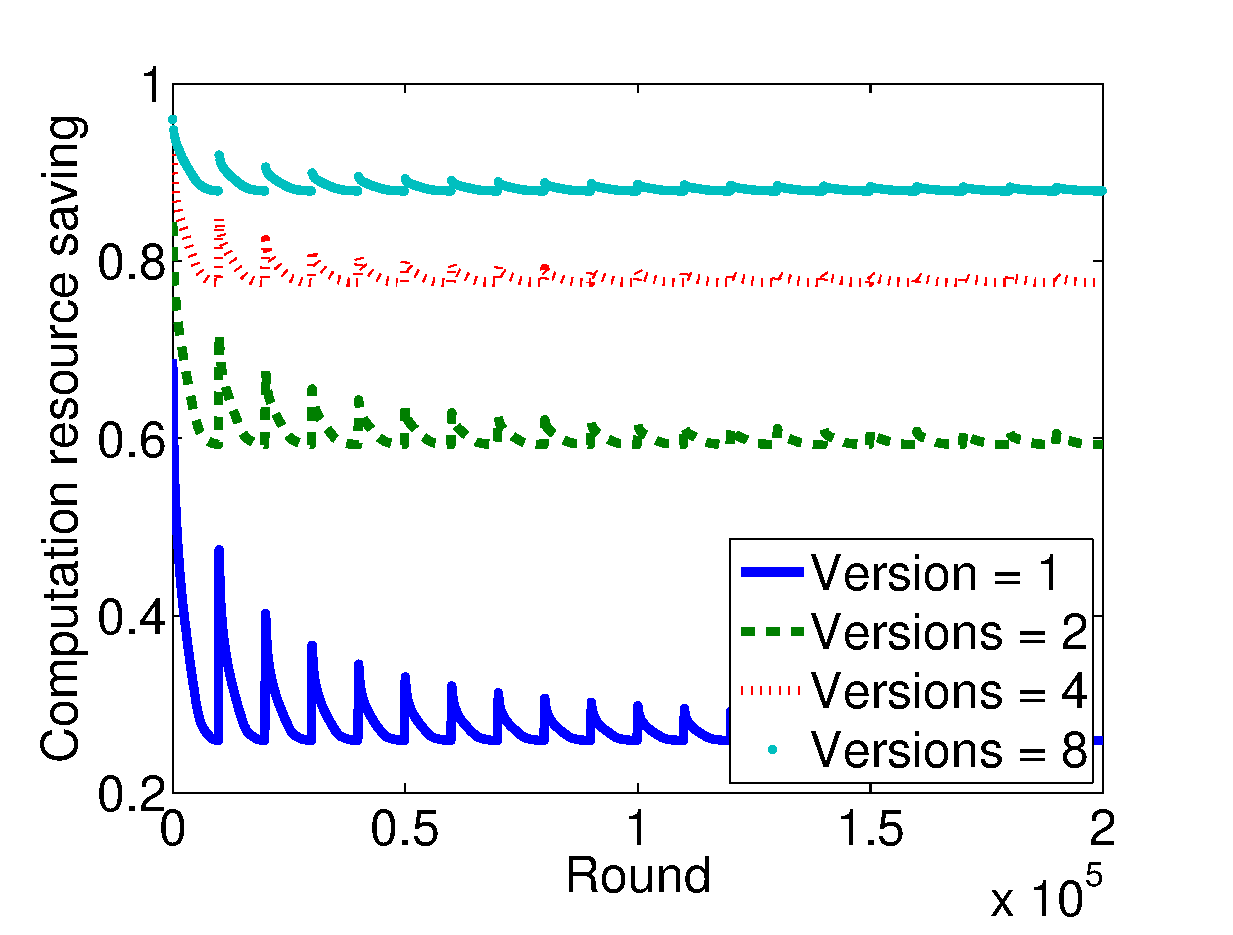
\includegraphics[width=0.33\linewidth]{fig/comp-saved-overtime-vs-ver-iter.eps}
			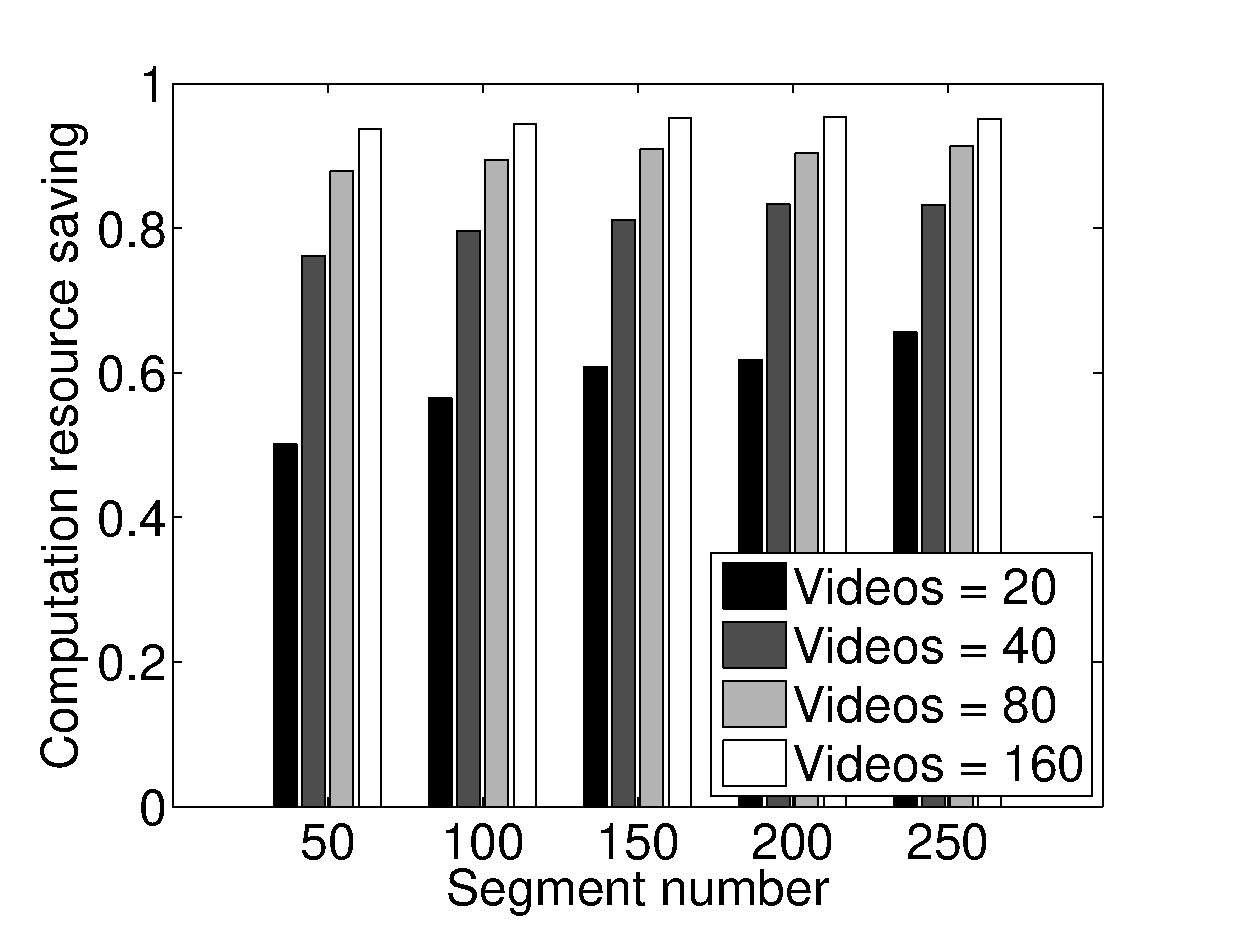
\includegraphics[width=0.33\linewidth]{fig/comp-saved-overtime-vs-vseg.eps}
		\item<1> Improvement of QoE\\
			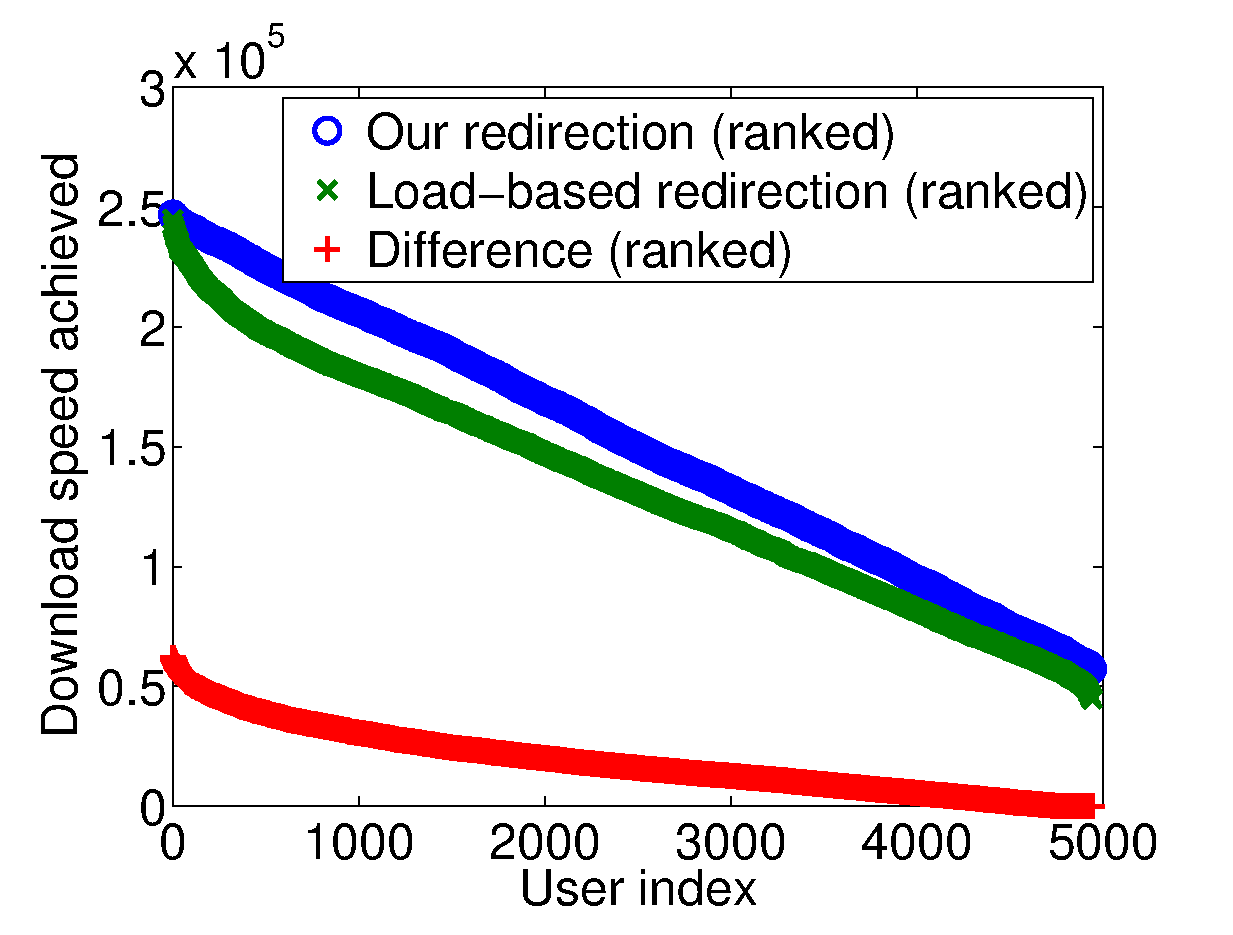
\includegraphics[width=0.33\linewidth]{fig/redirection-cmp.eps}
			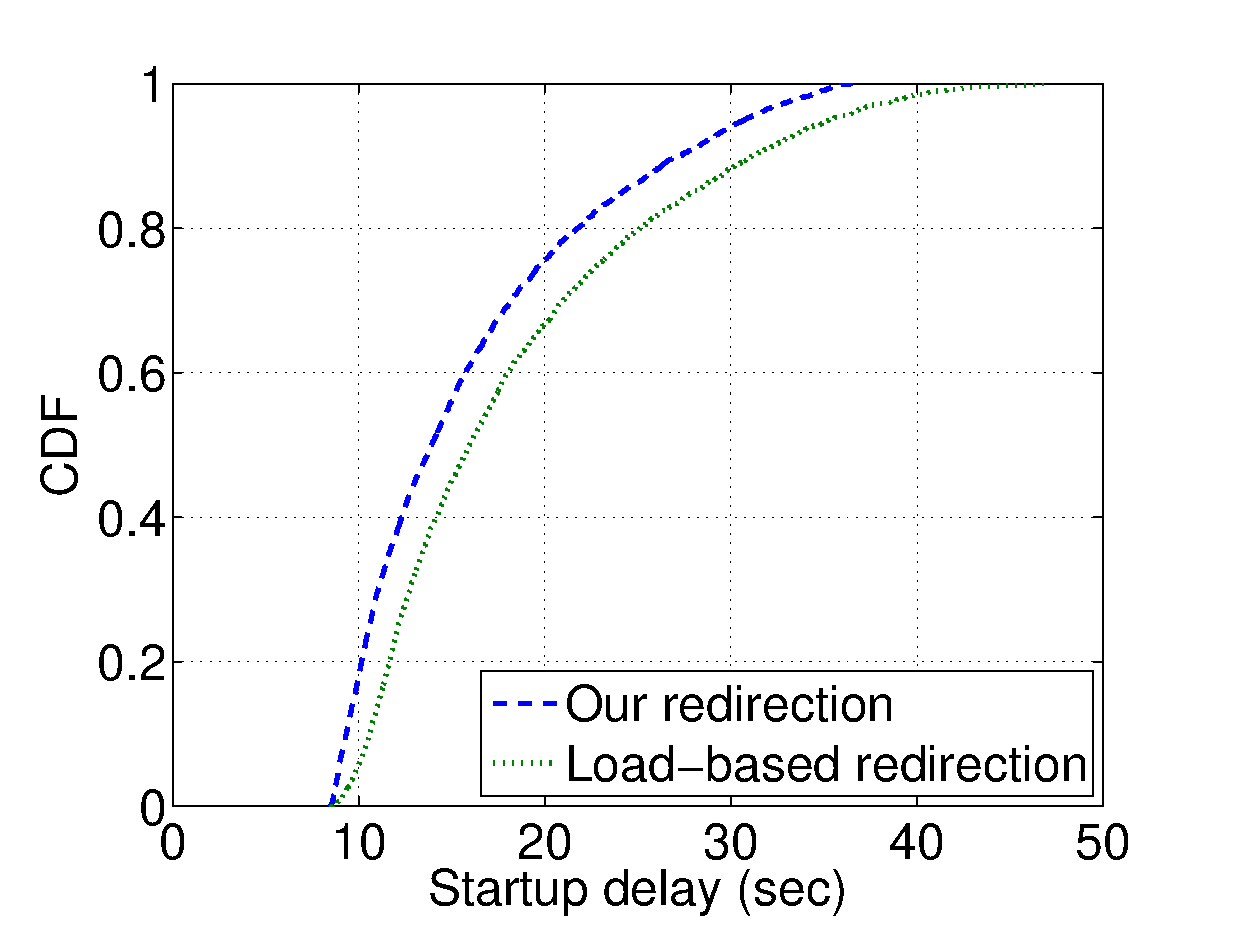
\includegraphics[width=0.33\linewidth]{fig/startup-delay.eps}
			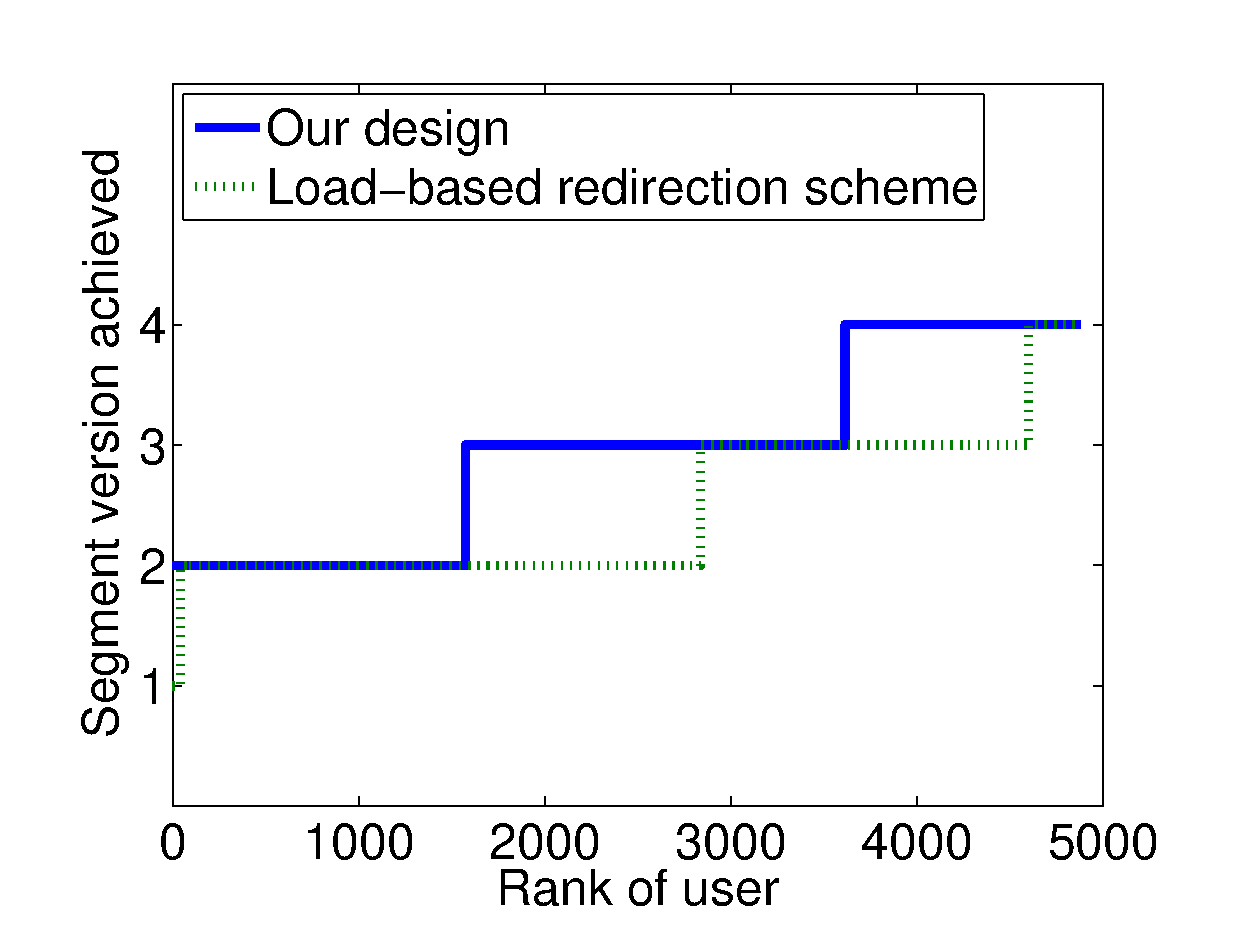
\includegraphics[width=0.33\linewidth]{fig/redirection-ver-cmp.eps}
	\end{itemize}
\end{frame}


\begin{frame}{Effects}
	\begin{itemize}
		\item<1> Mismatch\\
		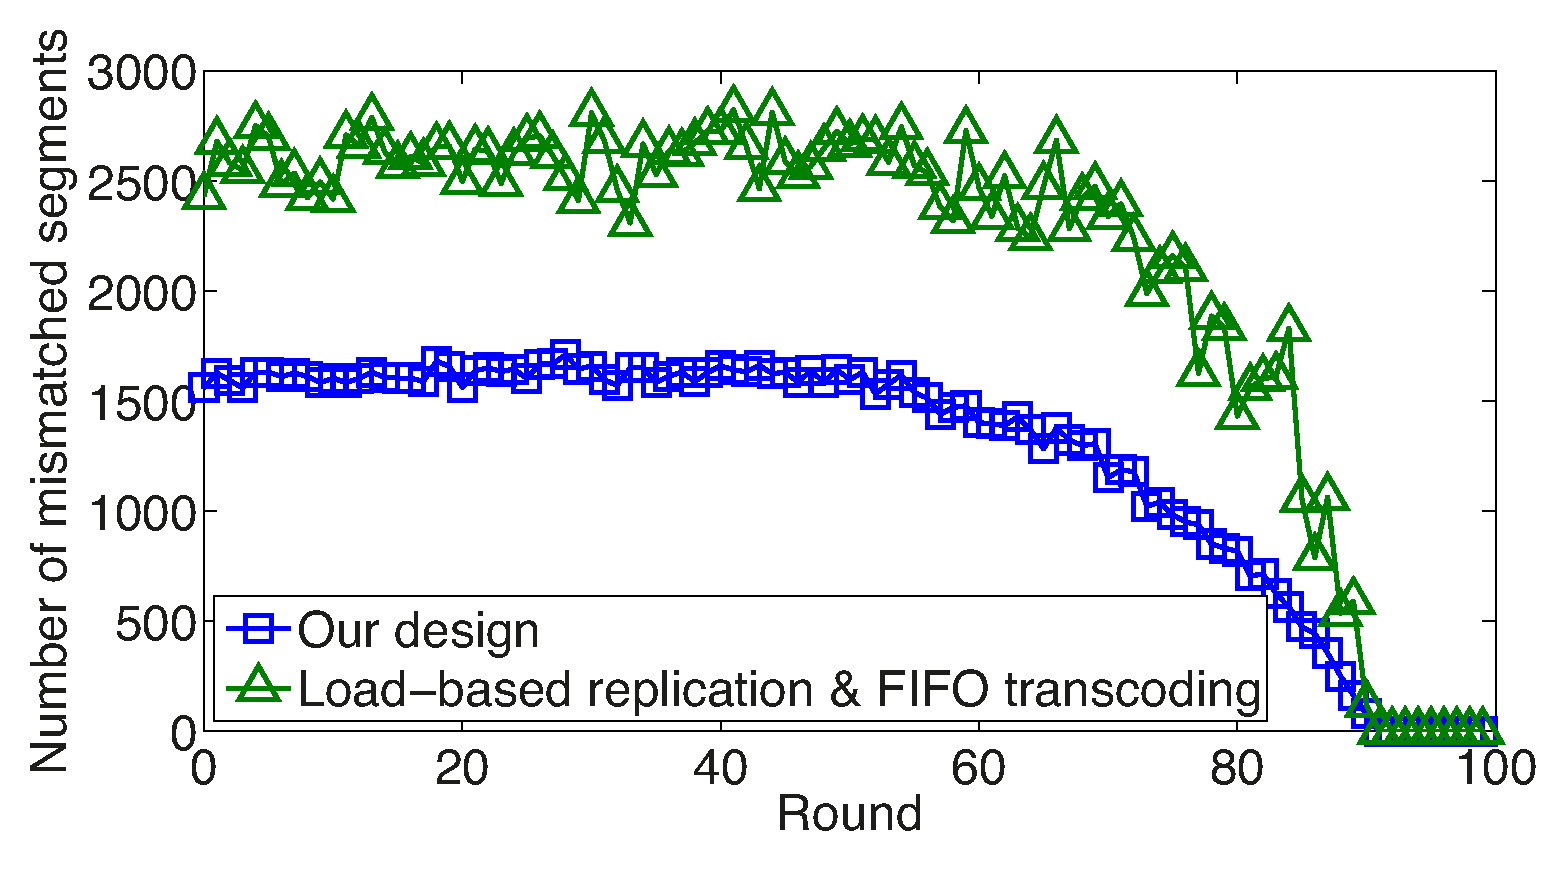
\includegraphics[width=0.44\linewidth]{fig/mismatch-overtime.eps}
		\item<1> Replication Cost\\
			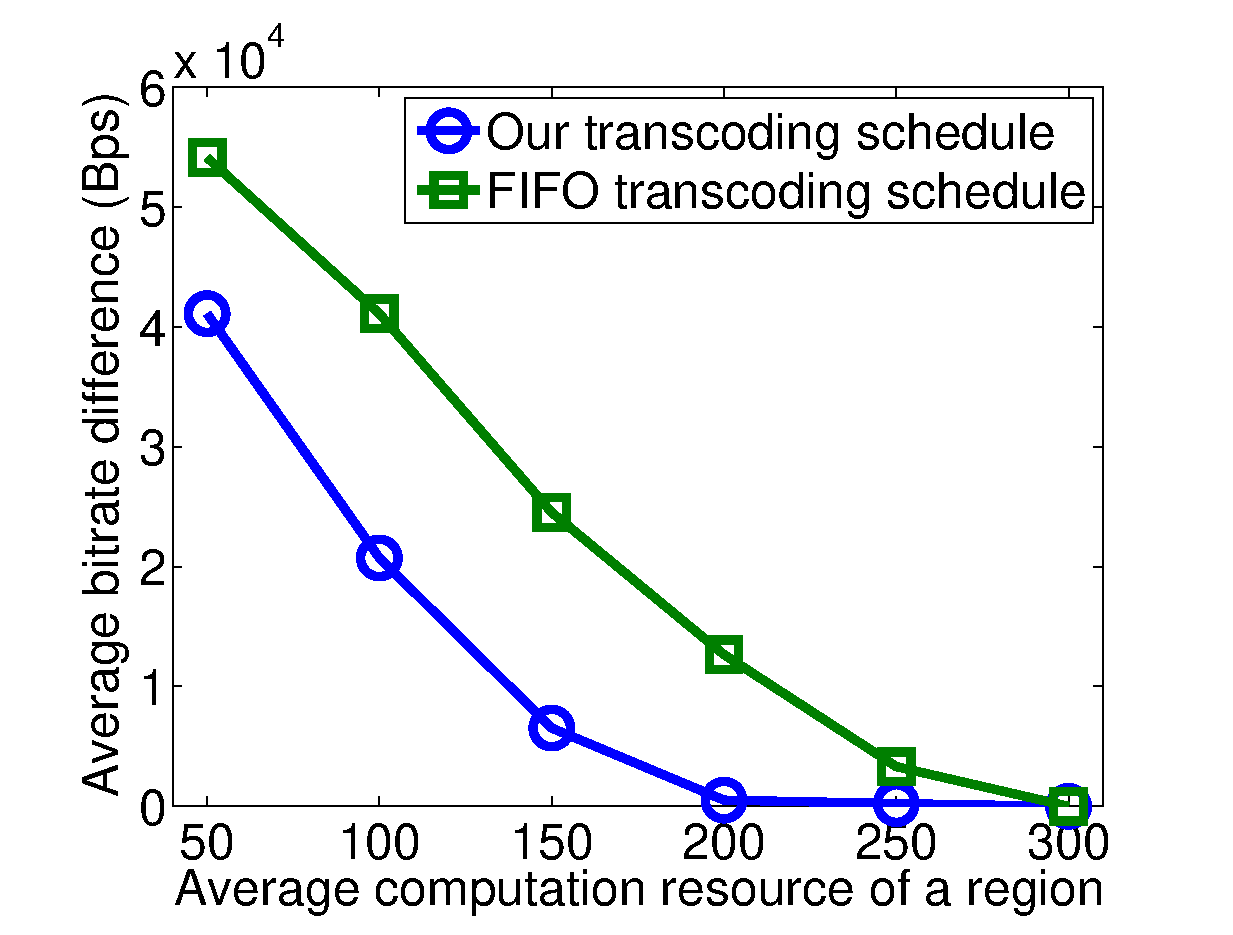
\includegraphics[width=0.45\linewidth]{fig/transcode-cmp-mismatchbit.eps}
			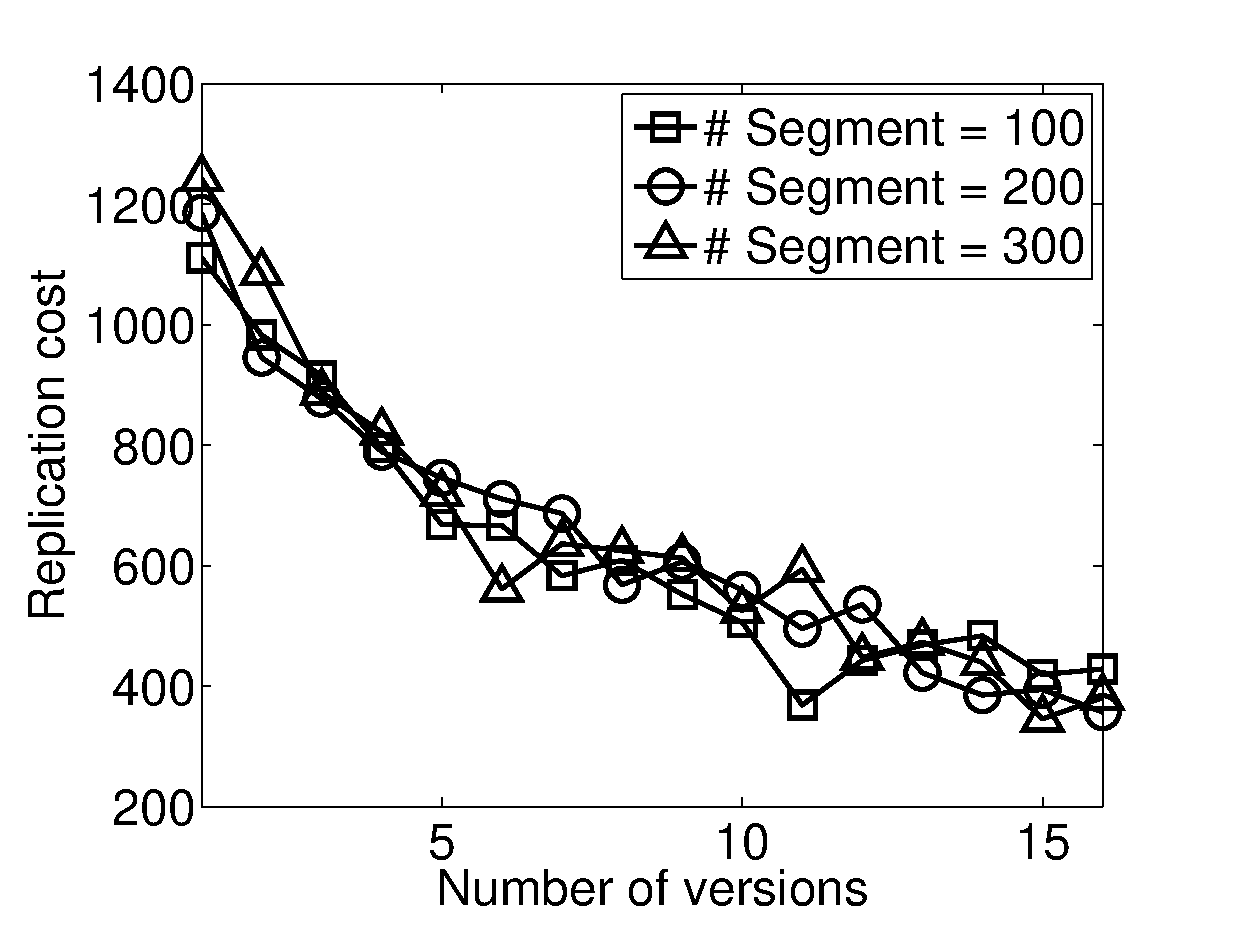
\includegraphics[width=0.45\linewidth]{fig/replication-cost-vs-version.eps}	
	\end{itemize}
\end{frame}

\begin{frame}{Effects}
	\begin{itemize}
		\item<1> Gap to the Optimal Solution\\
		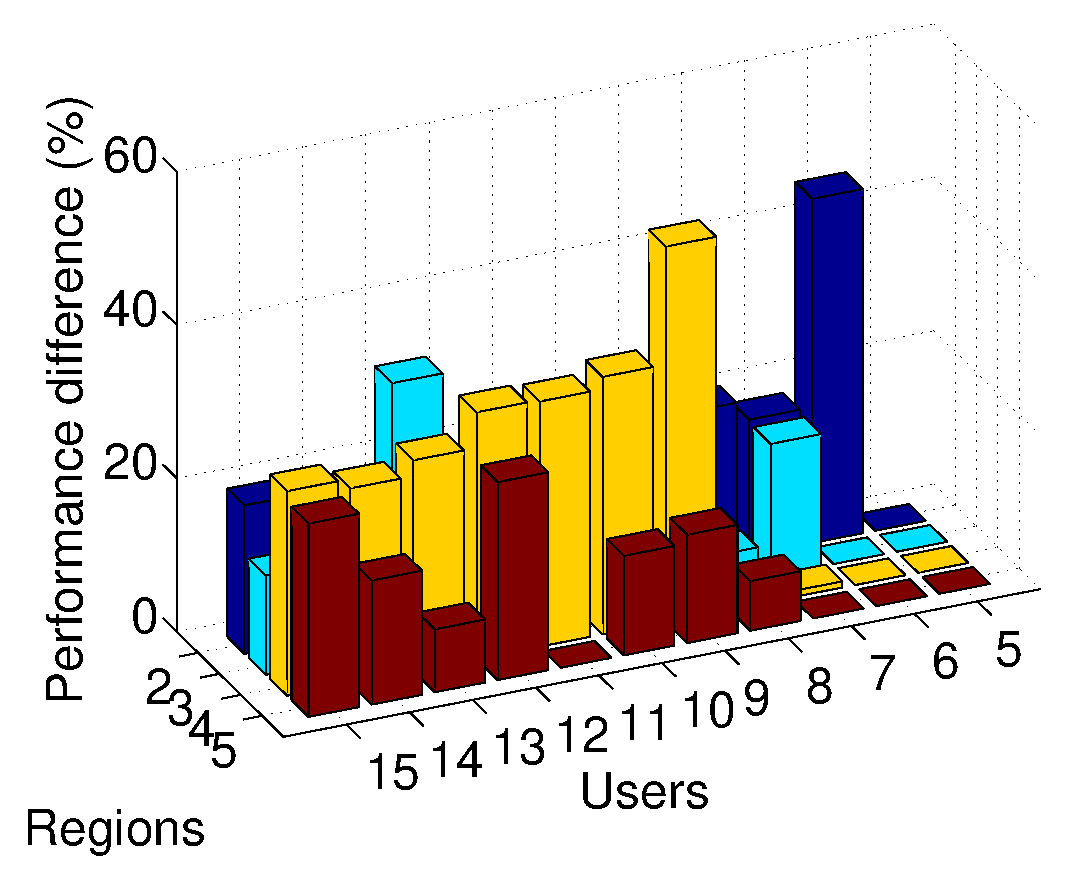
\includegraphics[width=0.72\linewidth]{fig/npproblem.eps}
	\end{itemize}
\end{frame}

\begin{frame}{Effects: Highlights}
	\begin{itemize}
		\item<1> $44.8\%$  users enjoy higher bitrate versions\\
		than the load-balanced redirection scheme
		\item<1> $4.5$x users enjoy the highest possible bitrate\\
		\item<1> Mismatch rate reduced by over $42.2\%$\\
		who receive a segment of a mismatched version
		\item<1> $\sim 80\%$ computing resource saved\\
		when the number of versions is 4. \\
		The higher the number is, the more resource our approach saves. 
	\end{itemize}
\end{frame}

\section{Conclusion}
\begin{frame}{Conclusion \& Q/A}
	Transcoding and Delivery can, and should be considered jointly. 
	\vskip 8ex
	Q/A?
\end{frame}

% -----------------------------------------------------------------------------
%\bibliographystyle{plainnat}
%\nobibligography{slides}
\end{document}